\documentclass[12pt,a4paper]{ctexart}
\usepackage[margin=2.2cm]{geometry}
\usepackage{graphicx}
\usepackage{booktabs}
\usepackage{amsmath}
\usepackage{float}
\usepackage{hyperref}
\usepackage{xcolor}
\usepackage{listings}

\lstset{
  basicstyle=\ttfamily\small,
  showstringspaces=false,
  breaklines=true,
  frame=single,
  tabsize=4
}

\newcommand{\reporttitle}{Tomasulo 算法仿真与实现}
\newcommand{\subtask}{Tomasulo 仿真器实现与分析}
\newcommand{\authname}{姓名}
\newcommand{\authid}{学号}

\title{\reporttitle}
\author{\authname：\underline{李祥熙} \quad \authid：\underline{2234412799}}
\date{\today}

\begin{document}
\maketitle
\tableofcontents
\newpage

\section{实验目的}
本实验的目标如下：
\begin{itemize}
  \item 加深对指令级并行性及其开发的理解；
  \item 加深对 Tomasulo 算法的理解；
  \item 掌握 Tomasulo 算法在指令流出、执行、写结果各阶段对浮点操作指令以及 load 和 store 指令进行的处理；
  \item 掌握采用 Tomasulo 算法的浮点处理部件的结构；
  \item 掌握保留站的结构；
  \item 给定被执行代码片段，能够在具体某个时钟周期写出保留站、指令状态表以及浮点寄存器状态表的变化情况。
\end{itemize}

\section{实验过程}
\subsection{实验环境}
\begin{itemize}
  \item 操作系统：macOS
  \item 编程语言：Python 3
  \item GUI 框架：PyQt5
\end{itemize}

\subsection{实现步骤}
主要实现流程如下：
\begin{enumerate}
  \item 设计仿真内核的数据结构：指令表示、指令状态表、保留站、寄存器状态和内存模型；
  \item 实现指令解析器，支持初始化语句（寄存器/内存赋值）和 MIPS 风格浮点指令：L.D, S.D, ADD.D, SUB.D, MUL.D, DIV.D；
  \item 实现发射（Issue）、开始执行（Start）、执行完成（End）和写结果（Write）四阶段的 Tomasulo 调度逻辑；
  \item 记录每周期的快照（CycleSnapshot），用于历史回放与 GUI 显示；
  \item 基于 PyQt5 实现交互界面，支持从编辑器或文件加载程序，单步/多步执行、运行到结束，以及历史回放的表格视图（保留站、指令状态、寄存器、内存）；
  \item 增加示例程序用于验证：无冲突、RAW、WAR 三类典型场景。
\end{enumerate}

\section{功能演示}

这一部份展现一些模拟器实现的功能。

\begin{figure}[H]
\centering
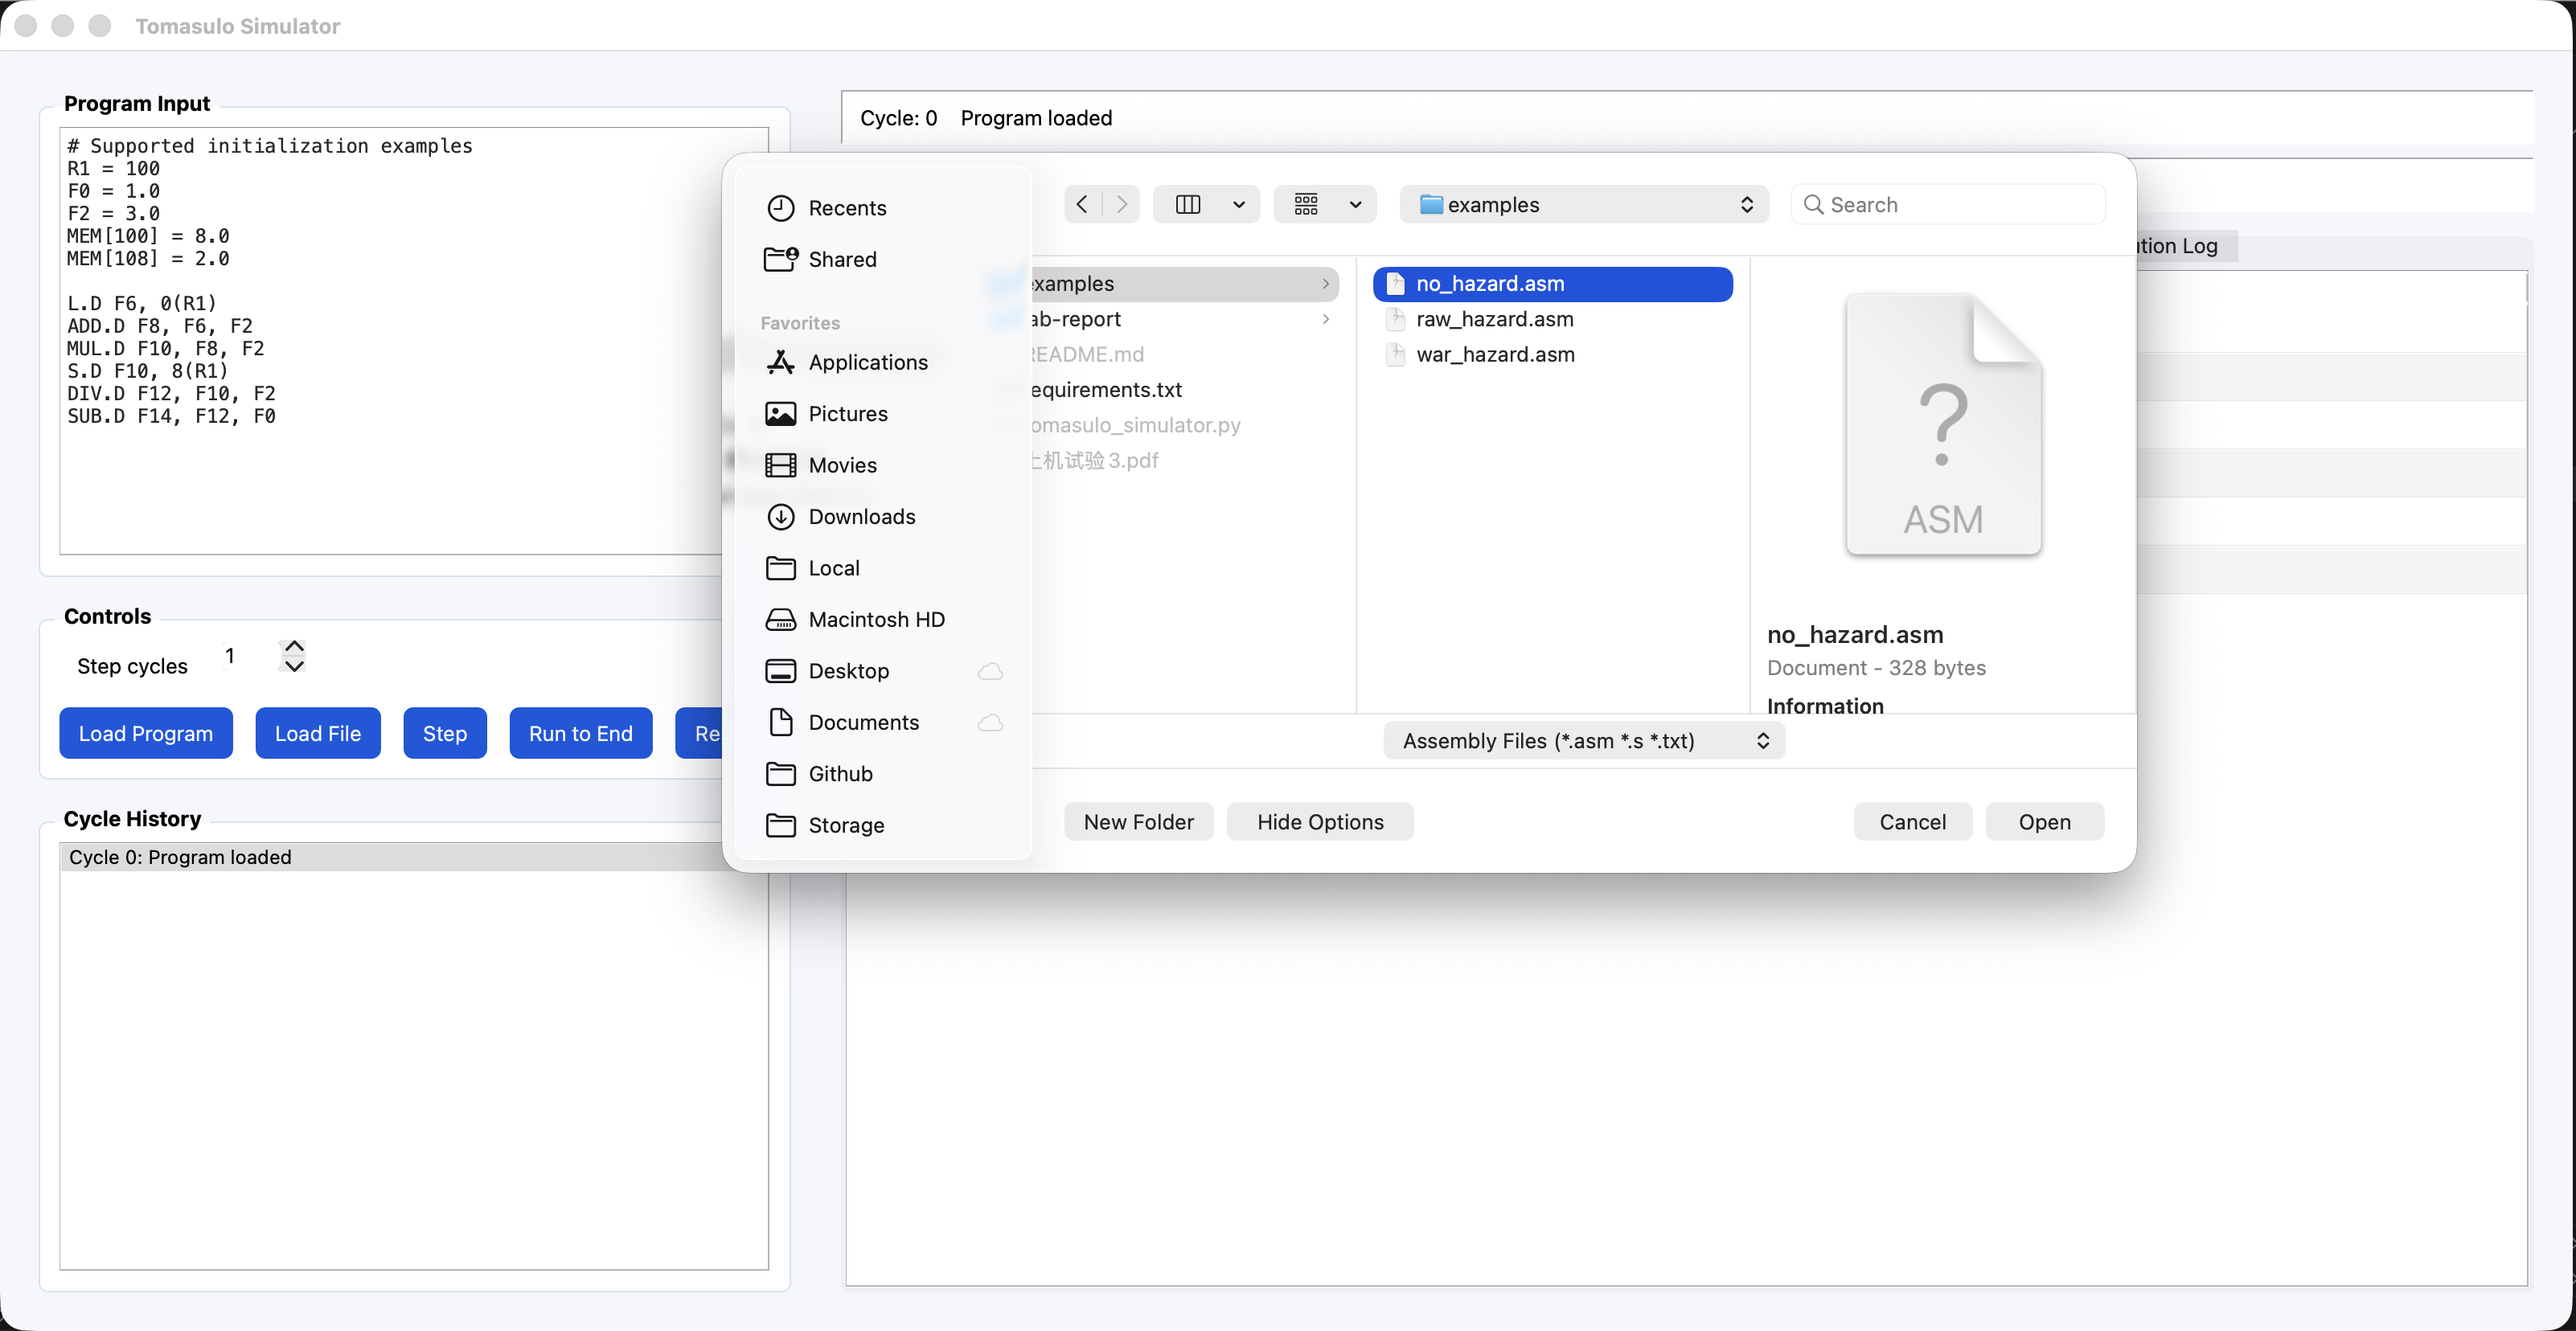
\includegraphics[width=0.8\textwidth]{images/0_import_from_file.png}
\caption{选择文件导入模拟器}
\end{figure}

\begin{figure}[H]
\centering
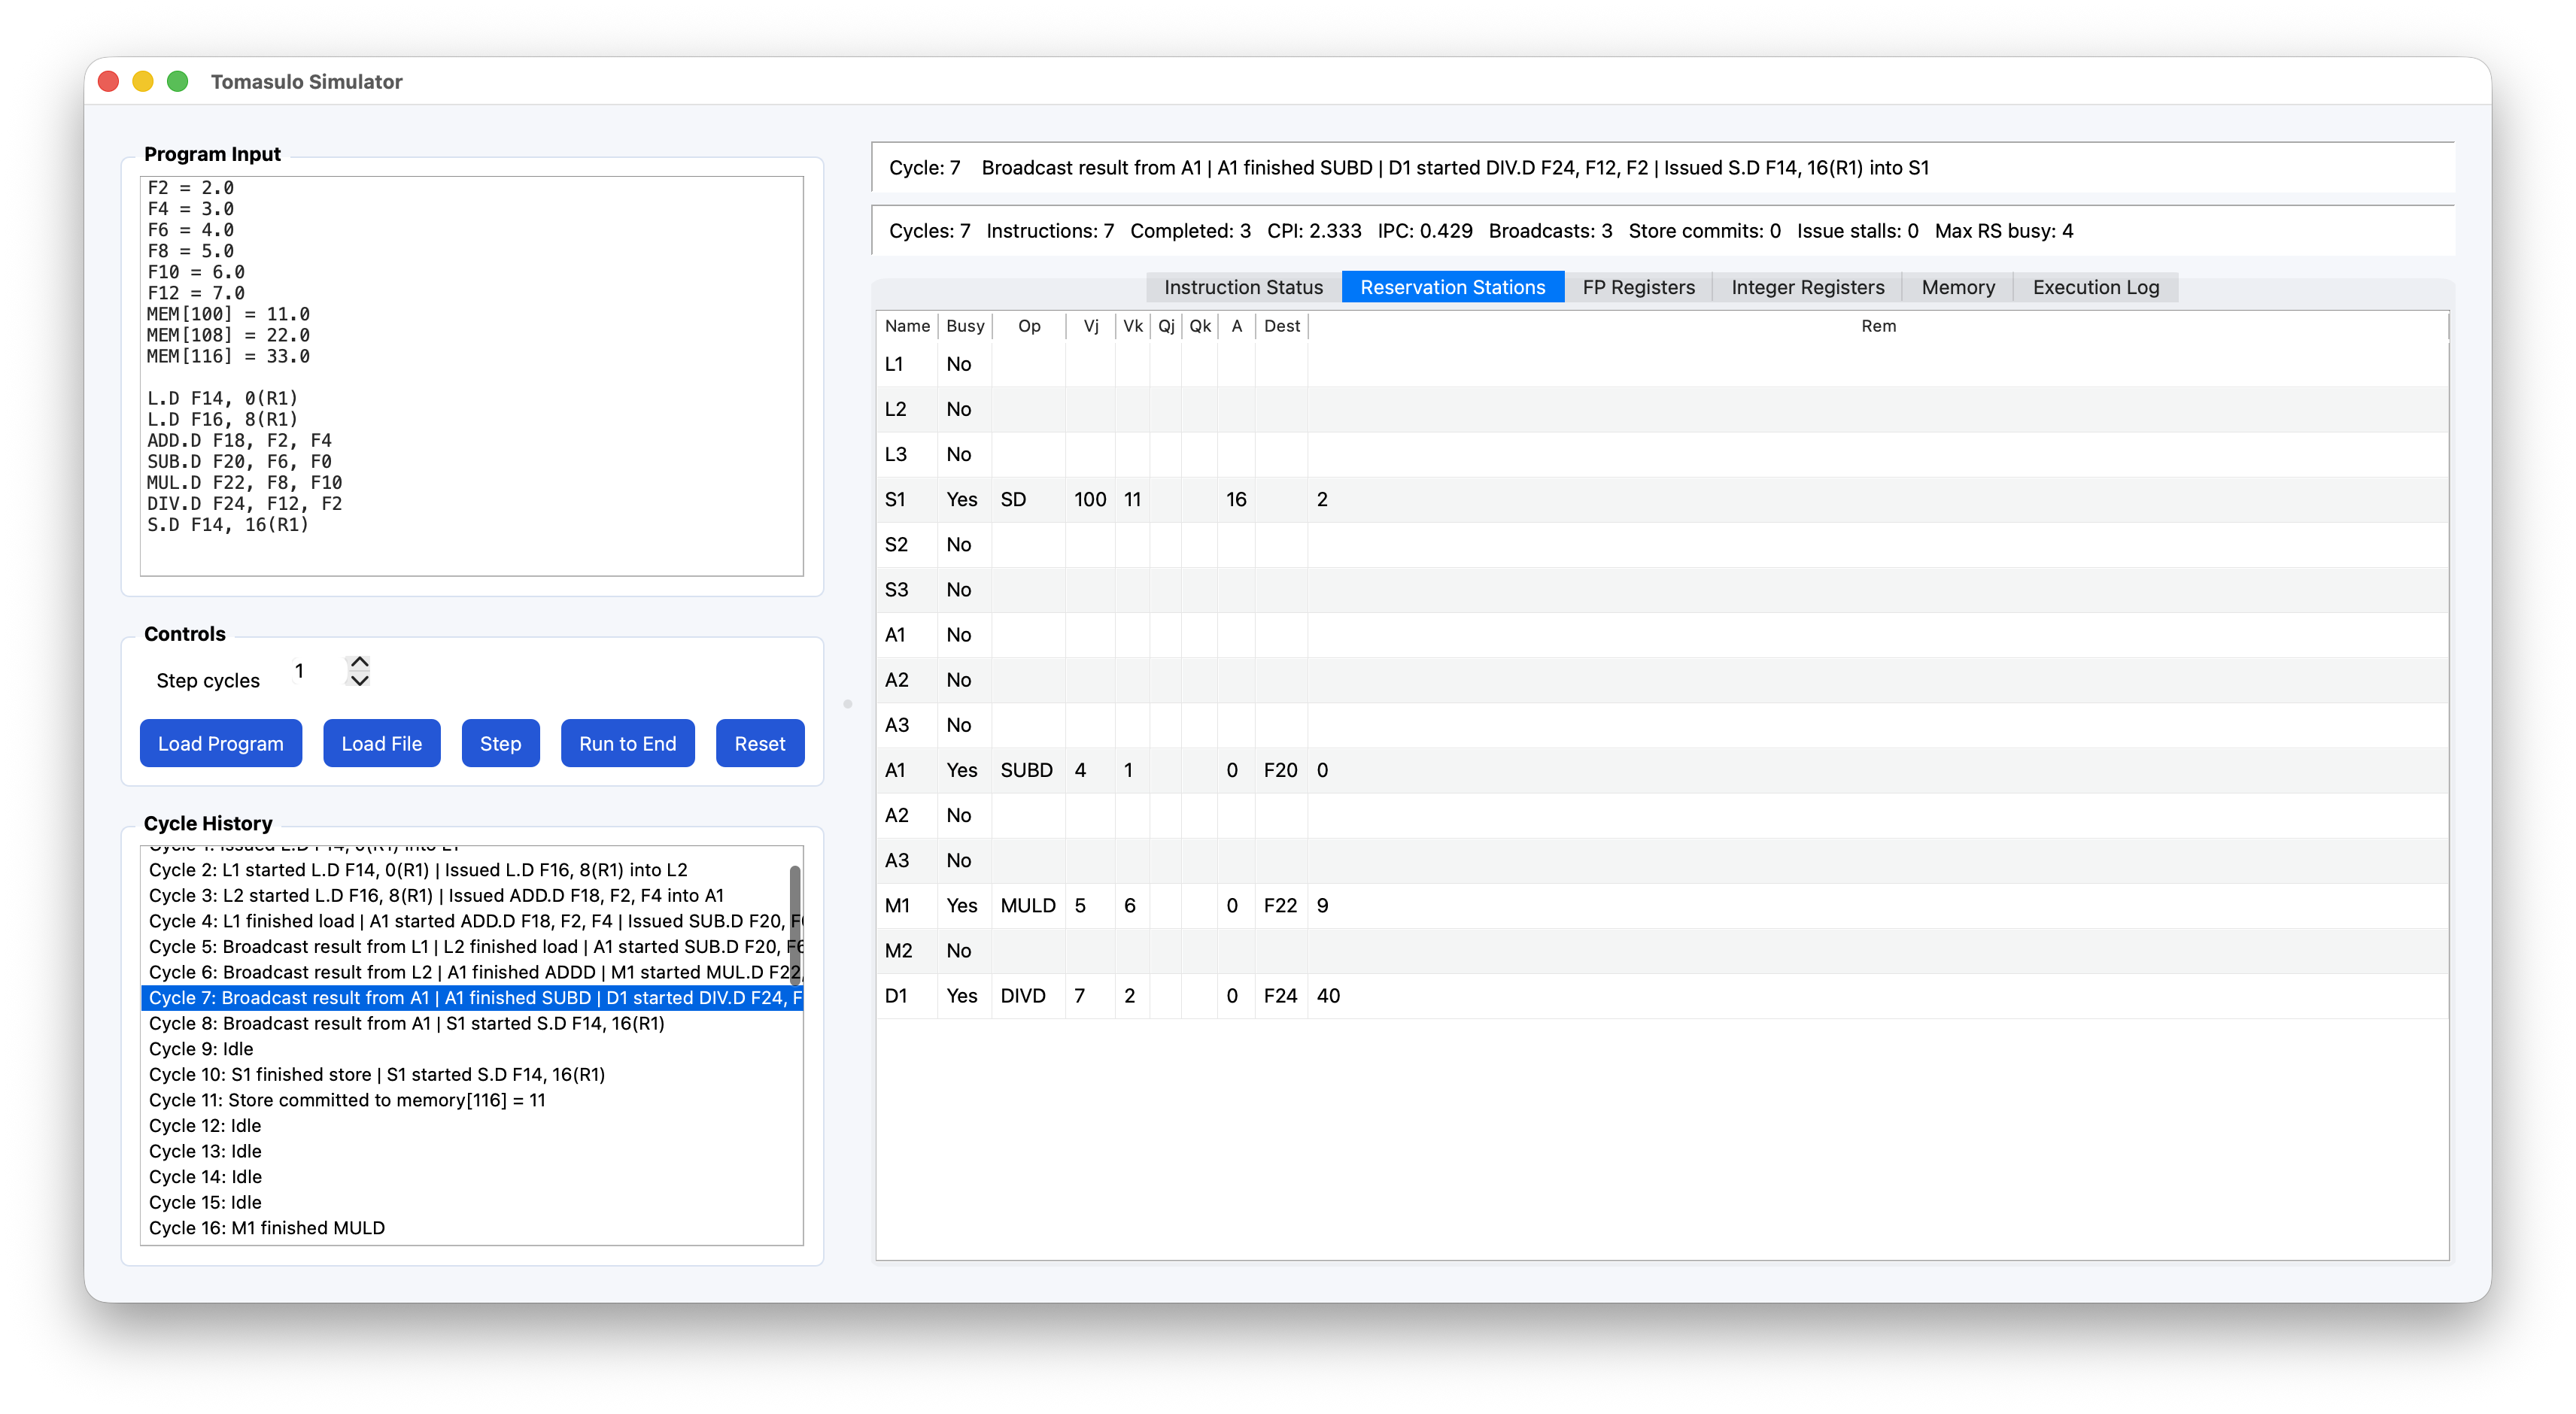
\includegraphics[width=0.8\textwidth]{images/3_replay_reservation_station.png}
\caption{回放时显示保留站信息}
\end{figure}

\begin{figure}[H]
\centering
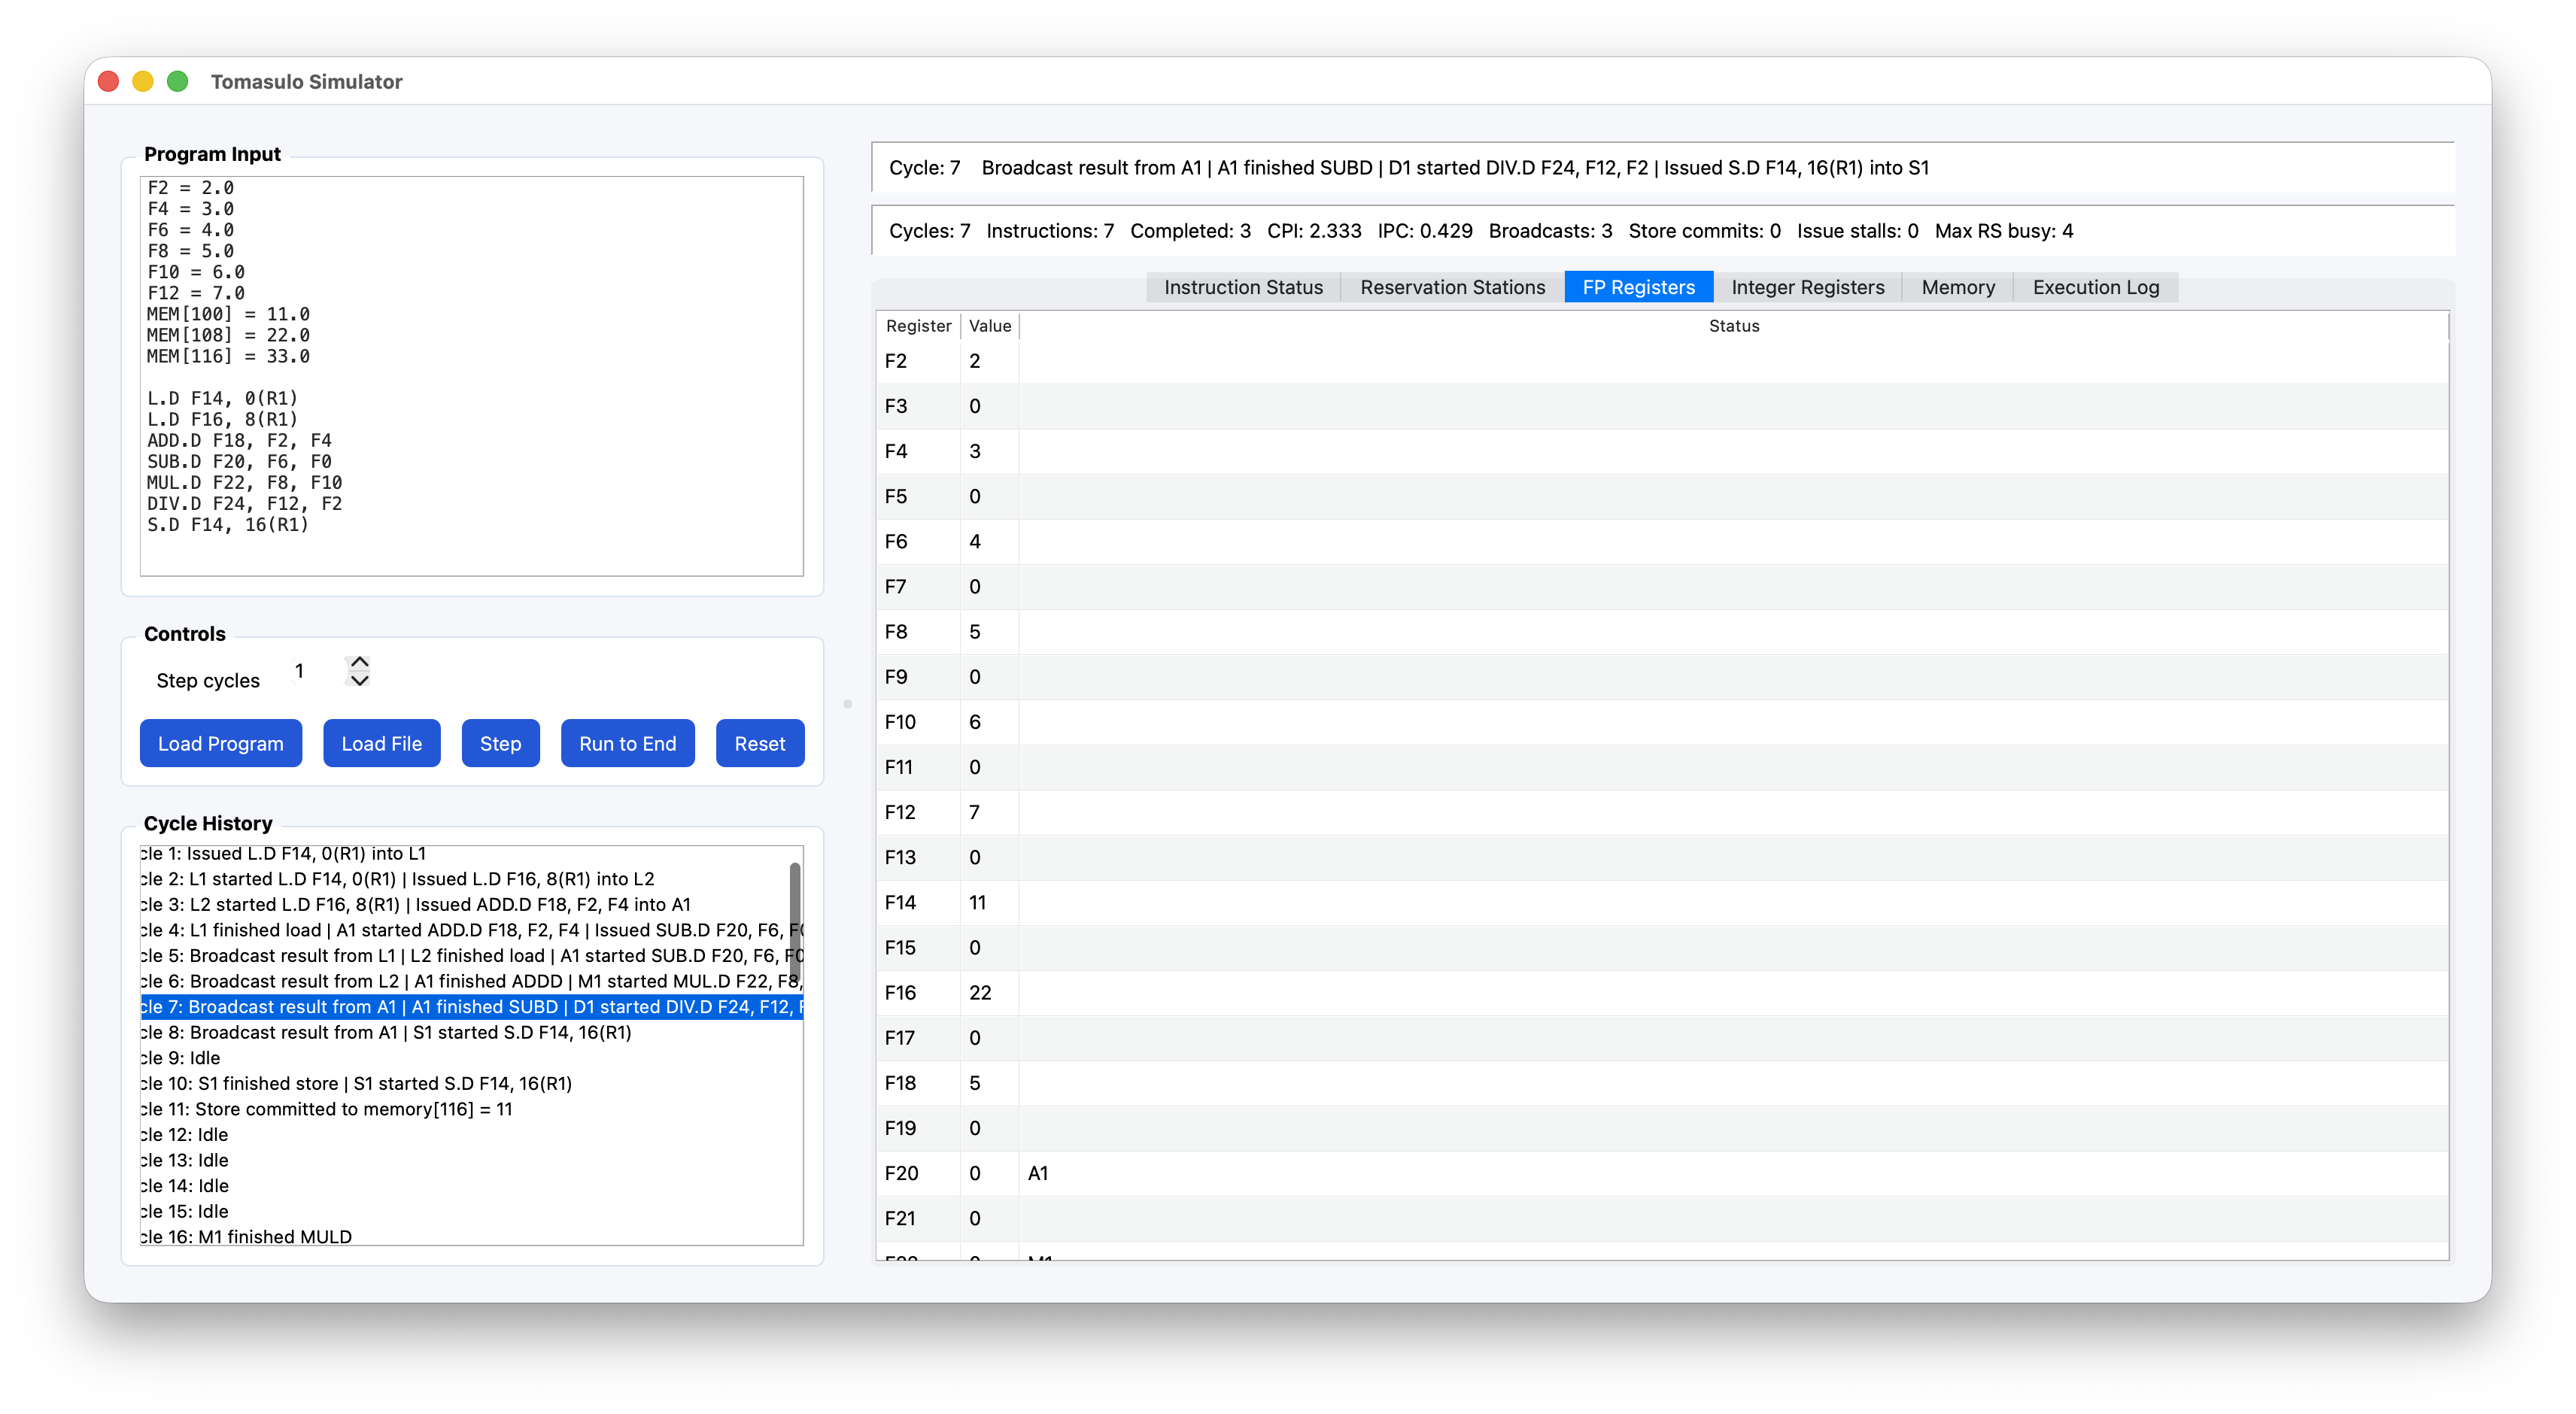
\includegraphics[width=0.8\textwidth]{images/4_replay_fp_regs.png}
\caption{回放时显示 FP 寄存器信息}
\end{figure}

\begin{figure}[H]
\centering
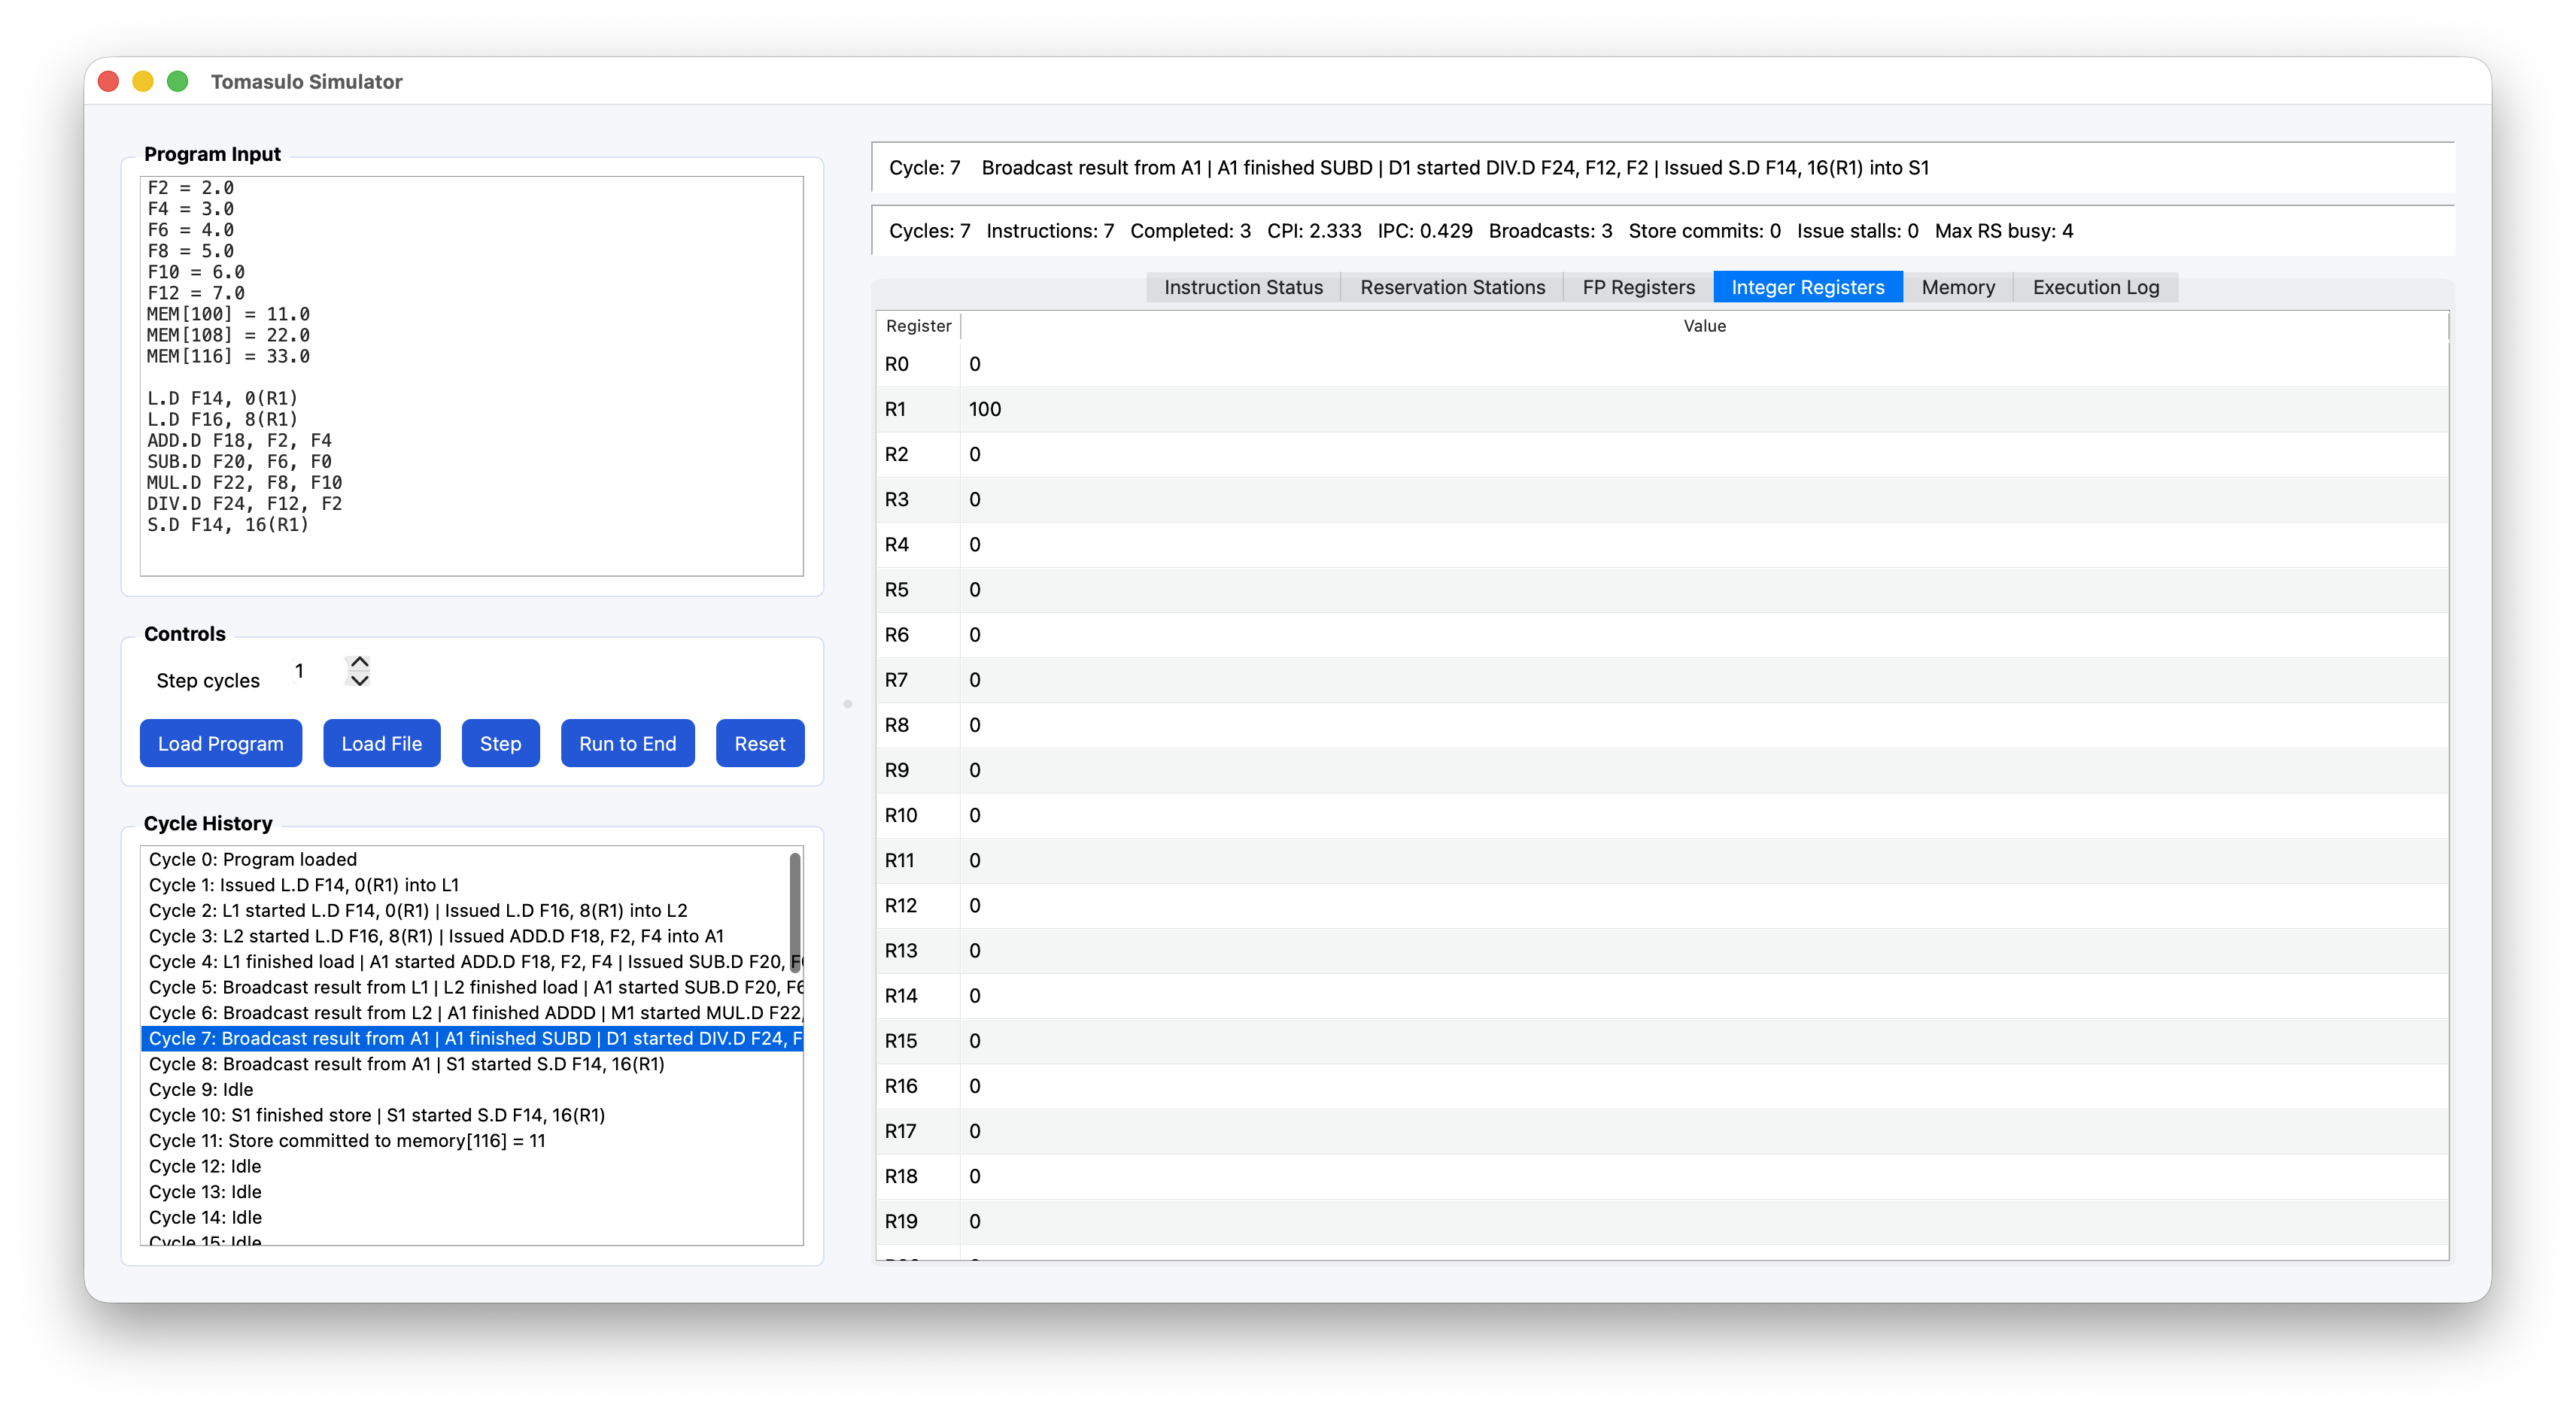
\includegraphics[width=0.8\textwidth]{images/5_replay_int_regs.png}
\caption{回放时显示整数寄存器信息}
\end{figure}

\begin{figure}[H]
\centering
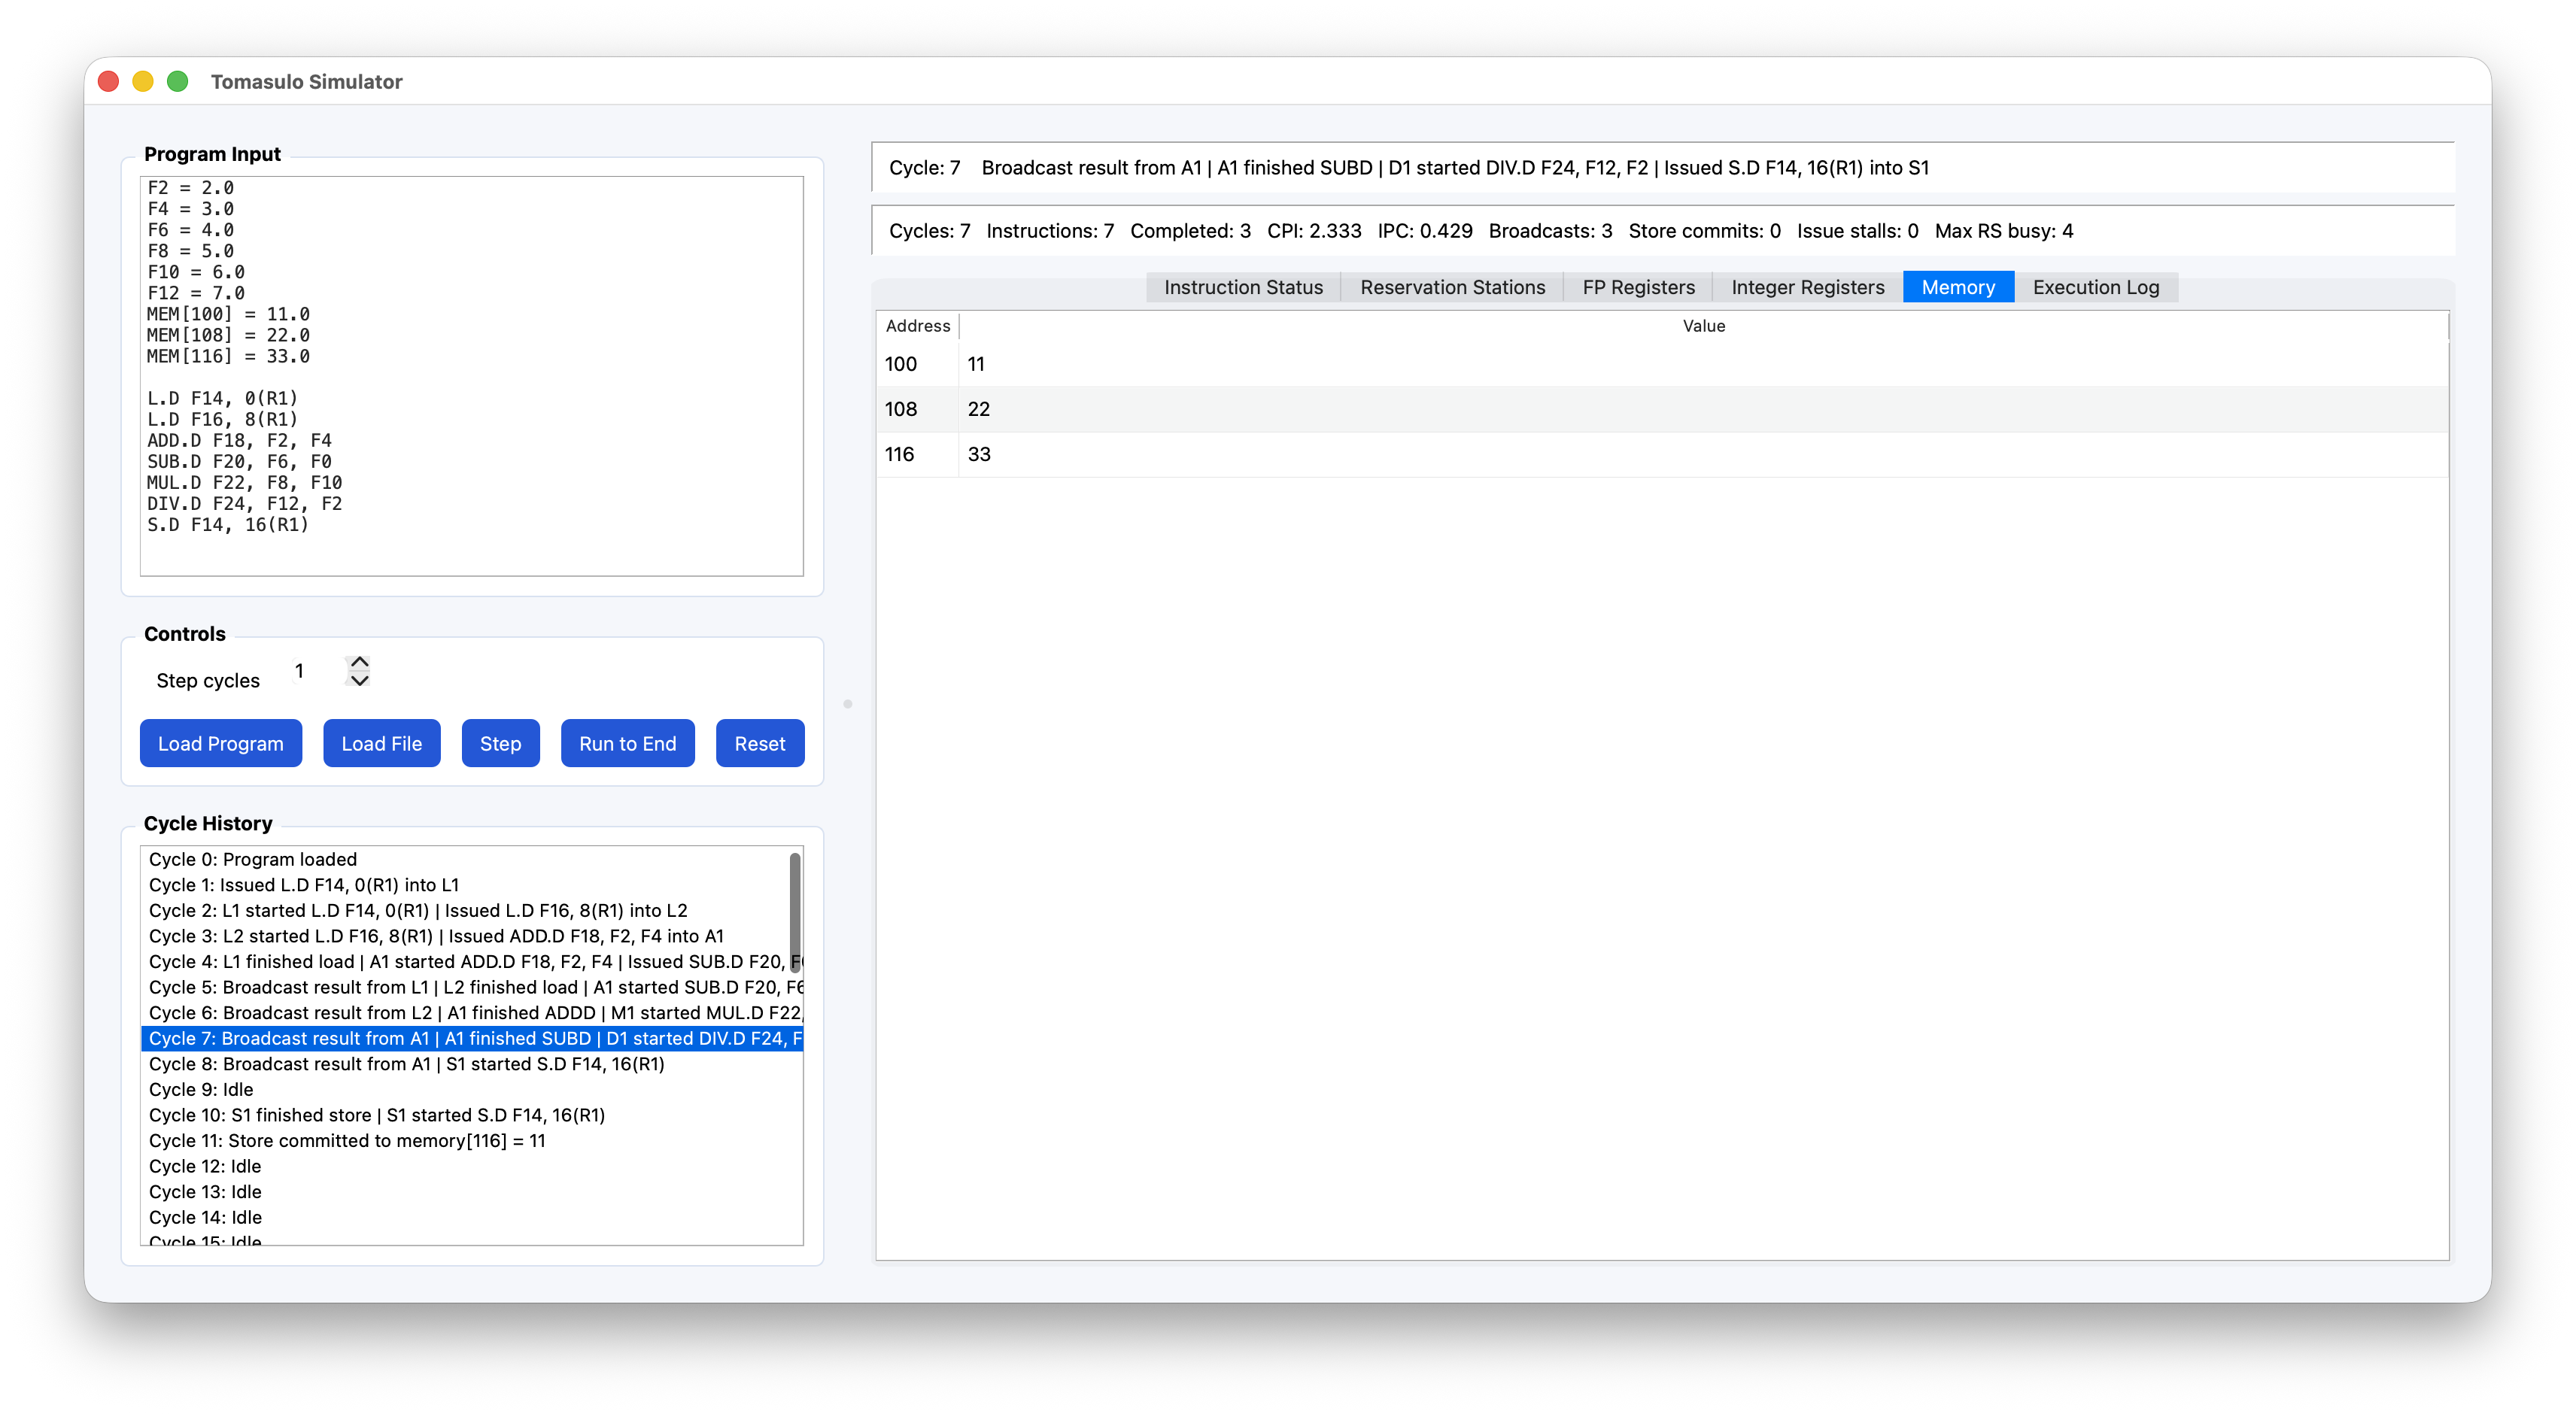
\includegraphics[width=0.8\textwidth]{images/6_replay_memory.png}
\caption{回放时显示内存信息}
\end{figure}

\begin{figure}[H]
\centering

\includegraphics[width=0.8\textwidth]{lab-report/images/7_paste_and_load.png}
\caption{粘贴代码到代码框并导入}
\end{figure}

\section{实验内容}
本次实验实现并测试了下列三个示例场景，分别用于展示 Tomasulo 仿真器在不同数据相关下的行为。

\subsection{示例一：无冲突 (No hazard)}
该示例包含相互独立的浮点运算与内存访问，用于演示在没有数据依赖时 Tomasulo 的流水并行性。示例代码如下：
\begin{lstlisting}
# No hazard sample
# Independent operations to demonstrate a clean Tomasulo schedule
R1 = 100
F0 = 1.0
F2 = 2.0
F4 = 3.0
F6 = 4.0
F8 = 5.0
F10 = 6.0
F12 = 7.0
MEM[100] = 11.0
MEM[108] = 22.0
MEM[116] = 33.0

L.D F14, 0(R1)
L.D F16, 8(R1)
ADD.D F18, F2, F4
SUB.D F20, F6, F0
MUL.D F22, F8, F10
DIV.D F24, F12, F2
S.D F14, 16(R1)
\end{lstlisting}

解释：本程序在初始化阶段设置了若干浮点寄存器与内存值，随后发出两条 load 指令和若干独立的浮点运算指令。由于各浮点运算互不依赖同一输入，保留站可以并行发射与执行，从而体现指令级并行性。

对应的运行界面截图（单步与运行到结束示例）：
\begin{figure}[H]
\centering
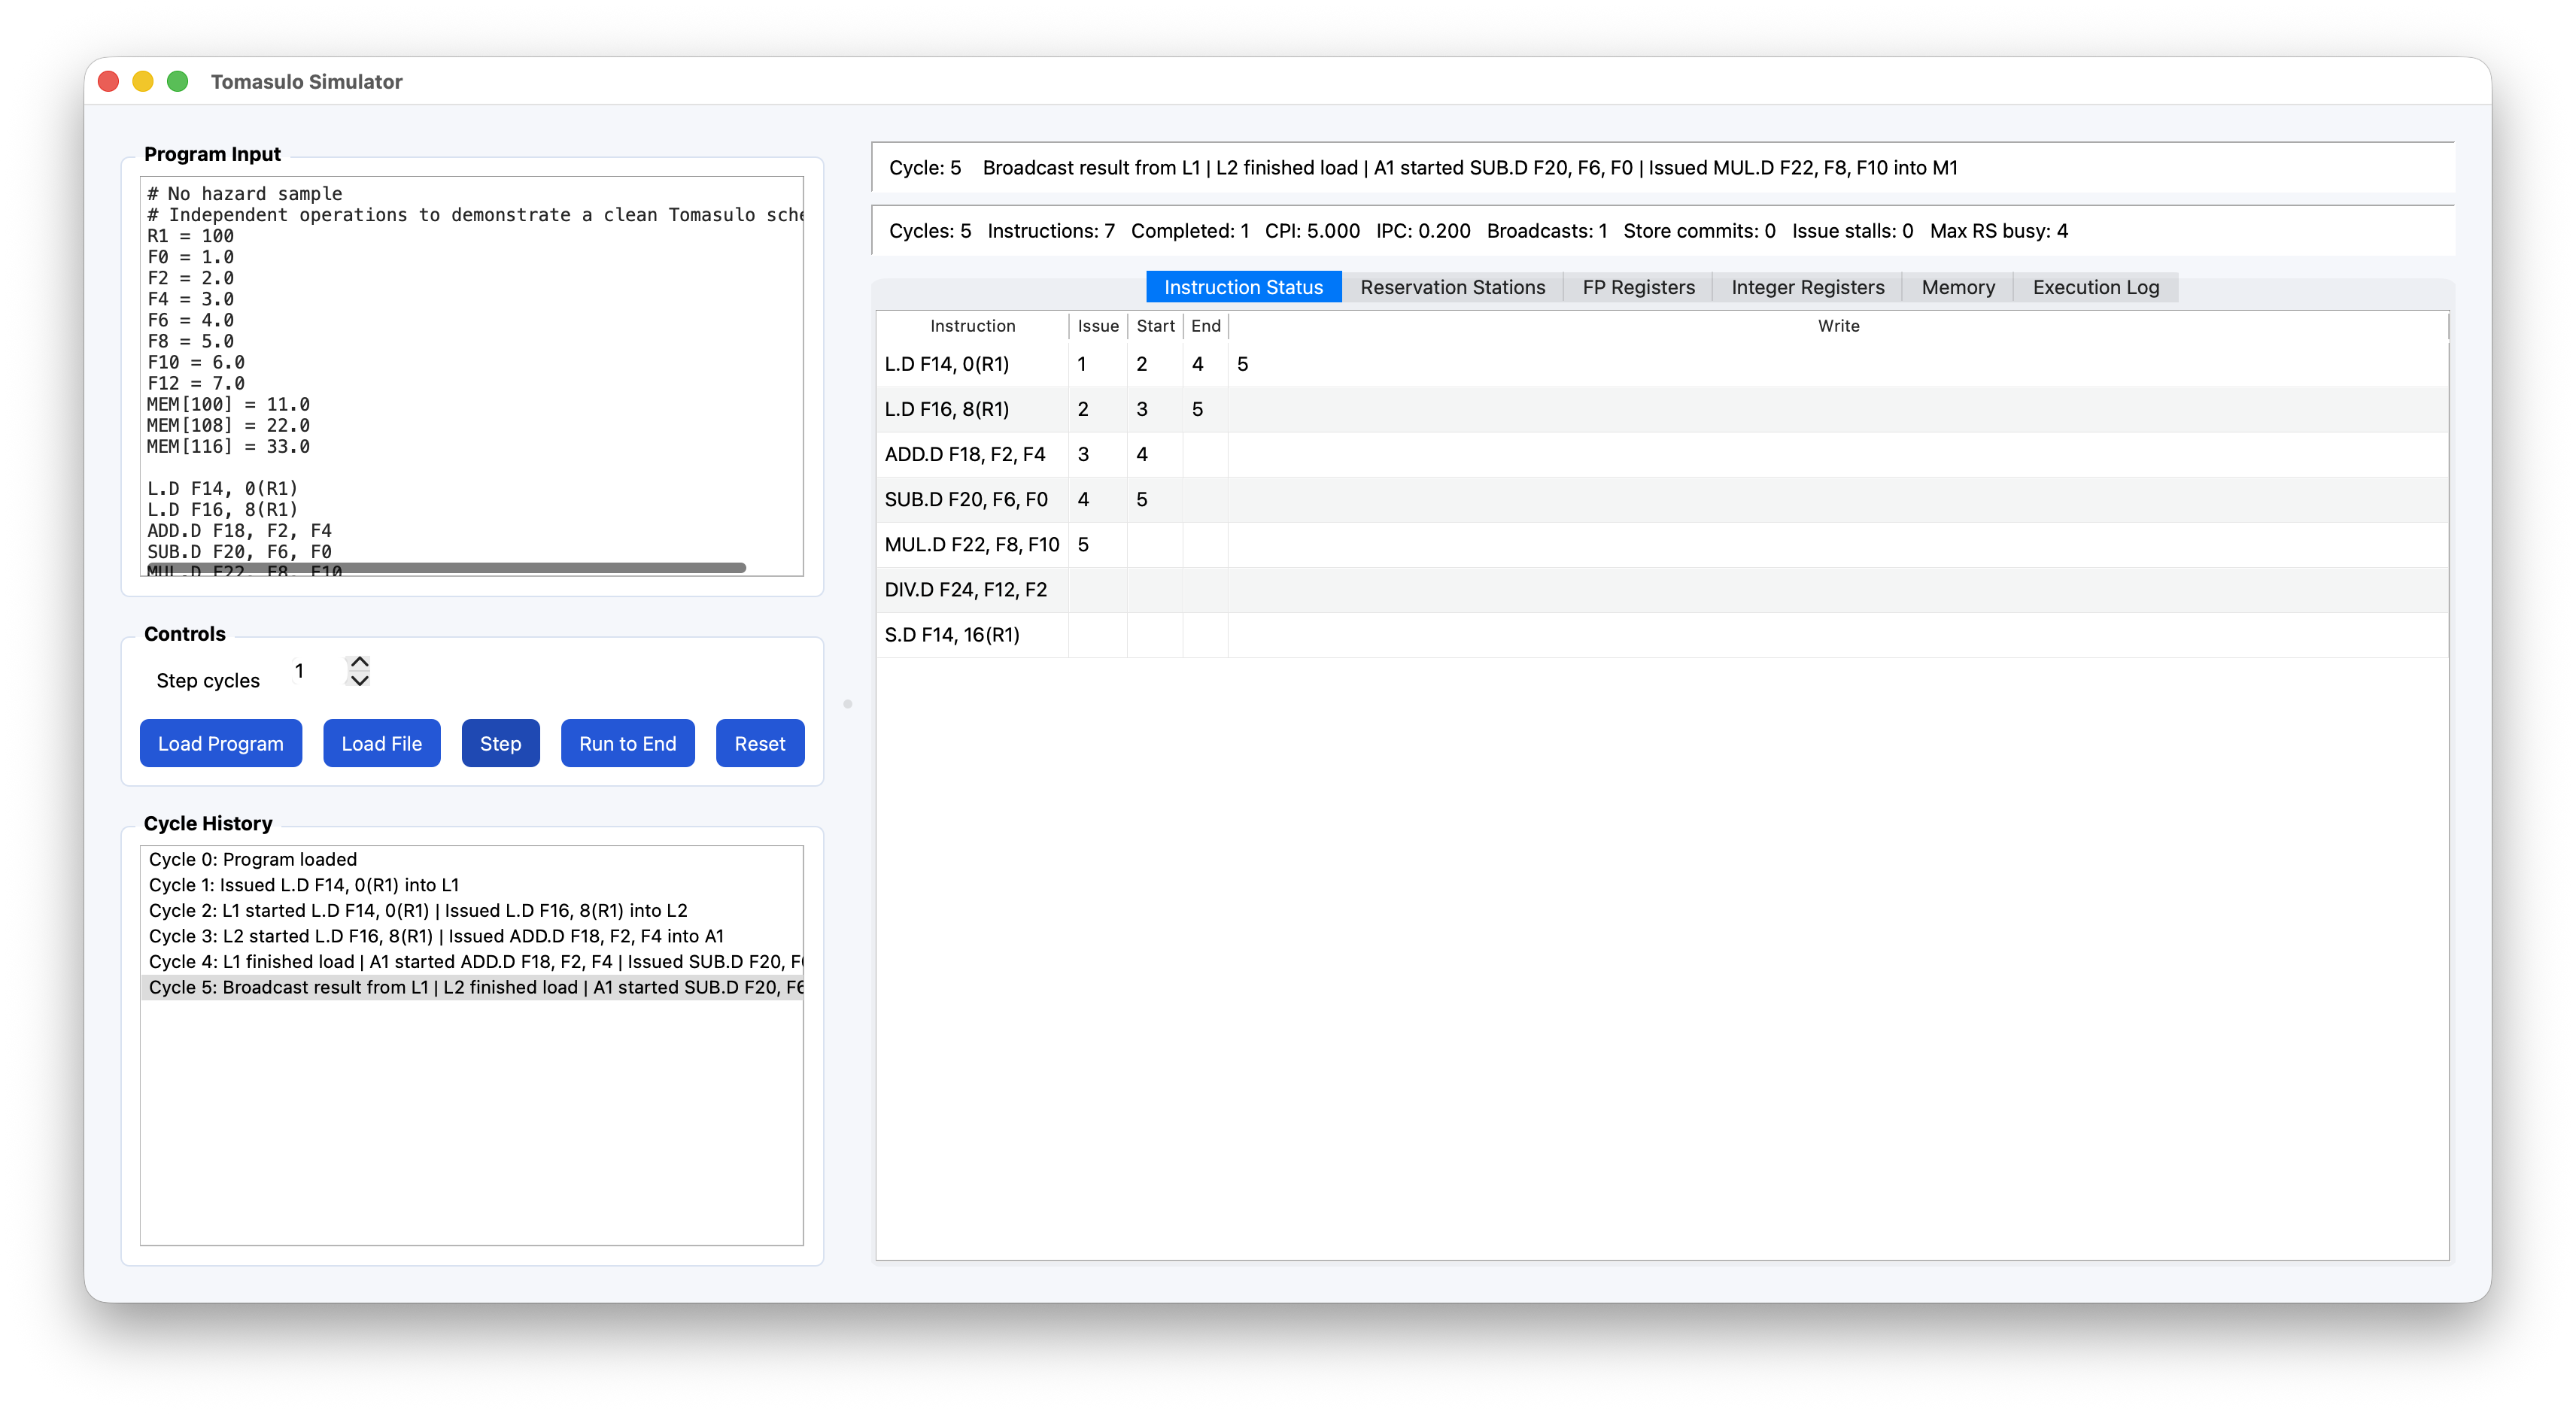
\includegraphics[width=0.8\textwidth]{images/1_step.png}
\caption{单步执行时的界面（示例：No hazard）}
\end{figure}

\begin{figure}[H]
\centering
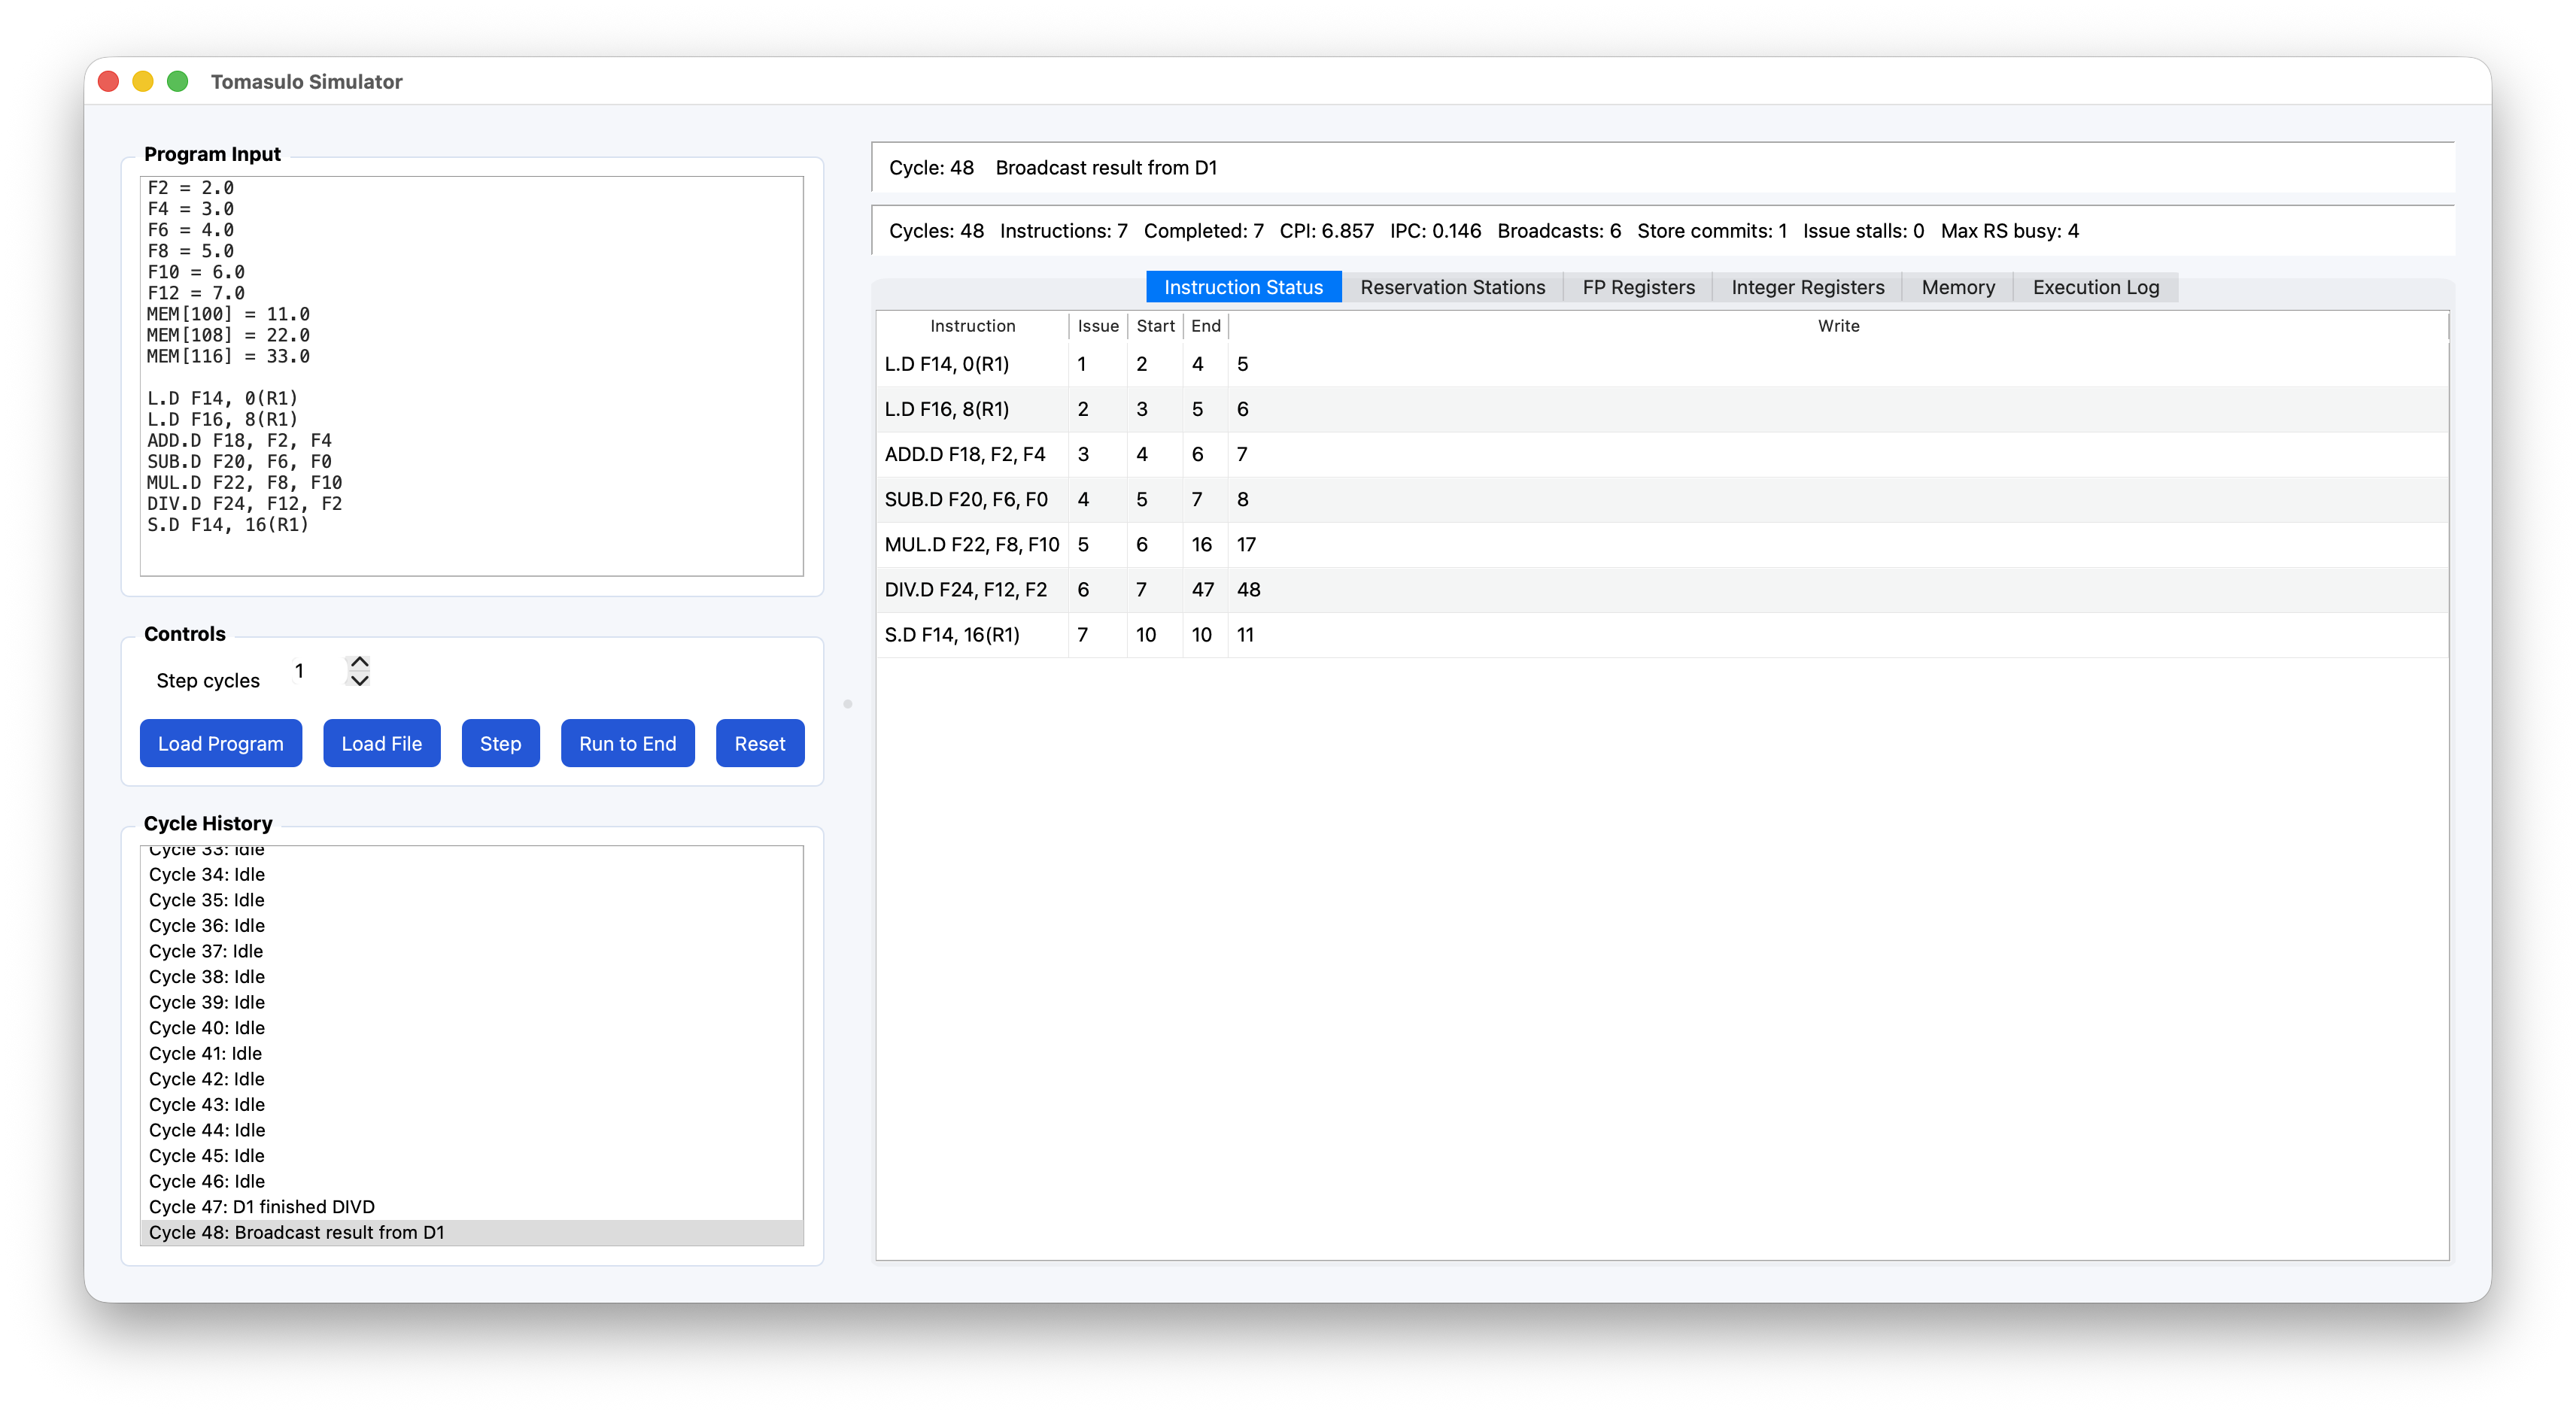
\includegraphics[width=0.8\textwidth]{images/2_run_to_end.png}
\caption{运行到结束后的快照（示例：No hazard）}
\end{figure}

\subsection{示例二：读后写（RAW）依赖}
该示例用于演示典型的读后写（Read After Write）数据相关：后续指令使用了前面 load 指令载入的数据，因而必须等待 load 写回并广播结果。示例代码如下：
\begin{lstlisting}
# RAW hazard sample
# F4 depends on the loaded value in F2
R1 = 100
F6 = 3.0
F8 = 5.0
MEM[100] = 8.0
MEM[108] = 4.0

L.D F2, 0(R1)
ADD.D F4, F2, F6
MUL.D F10, F4, F8
SUB.D F12, F10, F6
S.D F12, 8(R1)
\end{lstlisting}

解释：当 L.D 将数据载入并在写结果阶段广播时，依赖它的 ADD.D 才能获得操作数（通过寄存器状态或保留站的 Qj/Qk 标记）。此示例可展示保留站中 Qj/Qk 的传播、广播（broadcast）以及随后寄存器状态的清除。对应 GUI 的历史回放截图见下：
\begin{figure}[H]
\centering
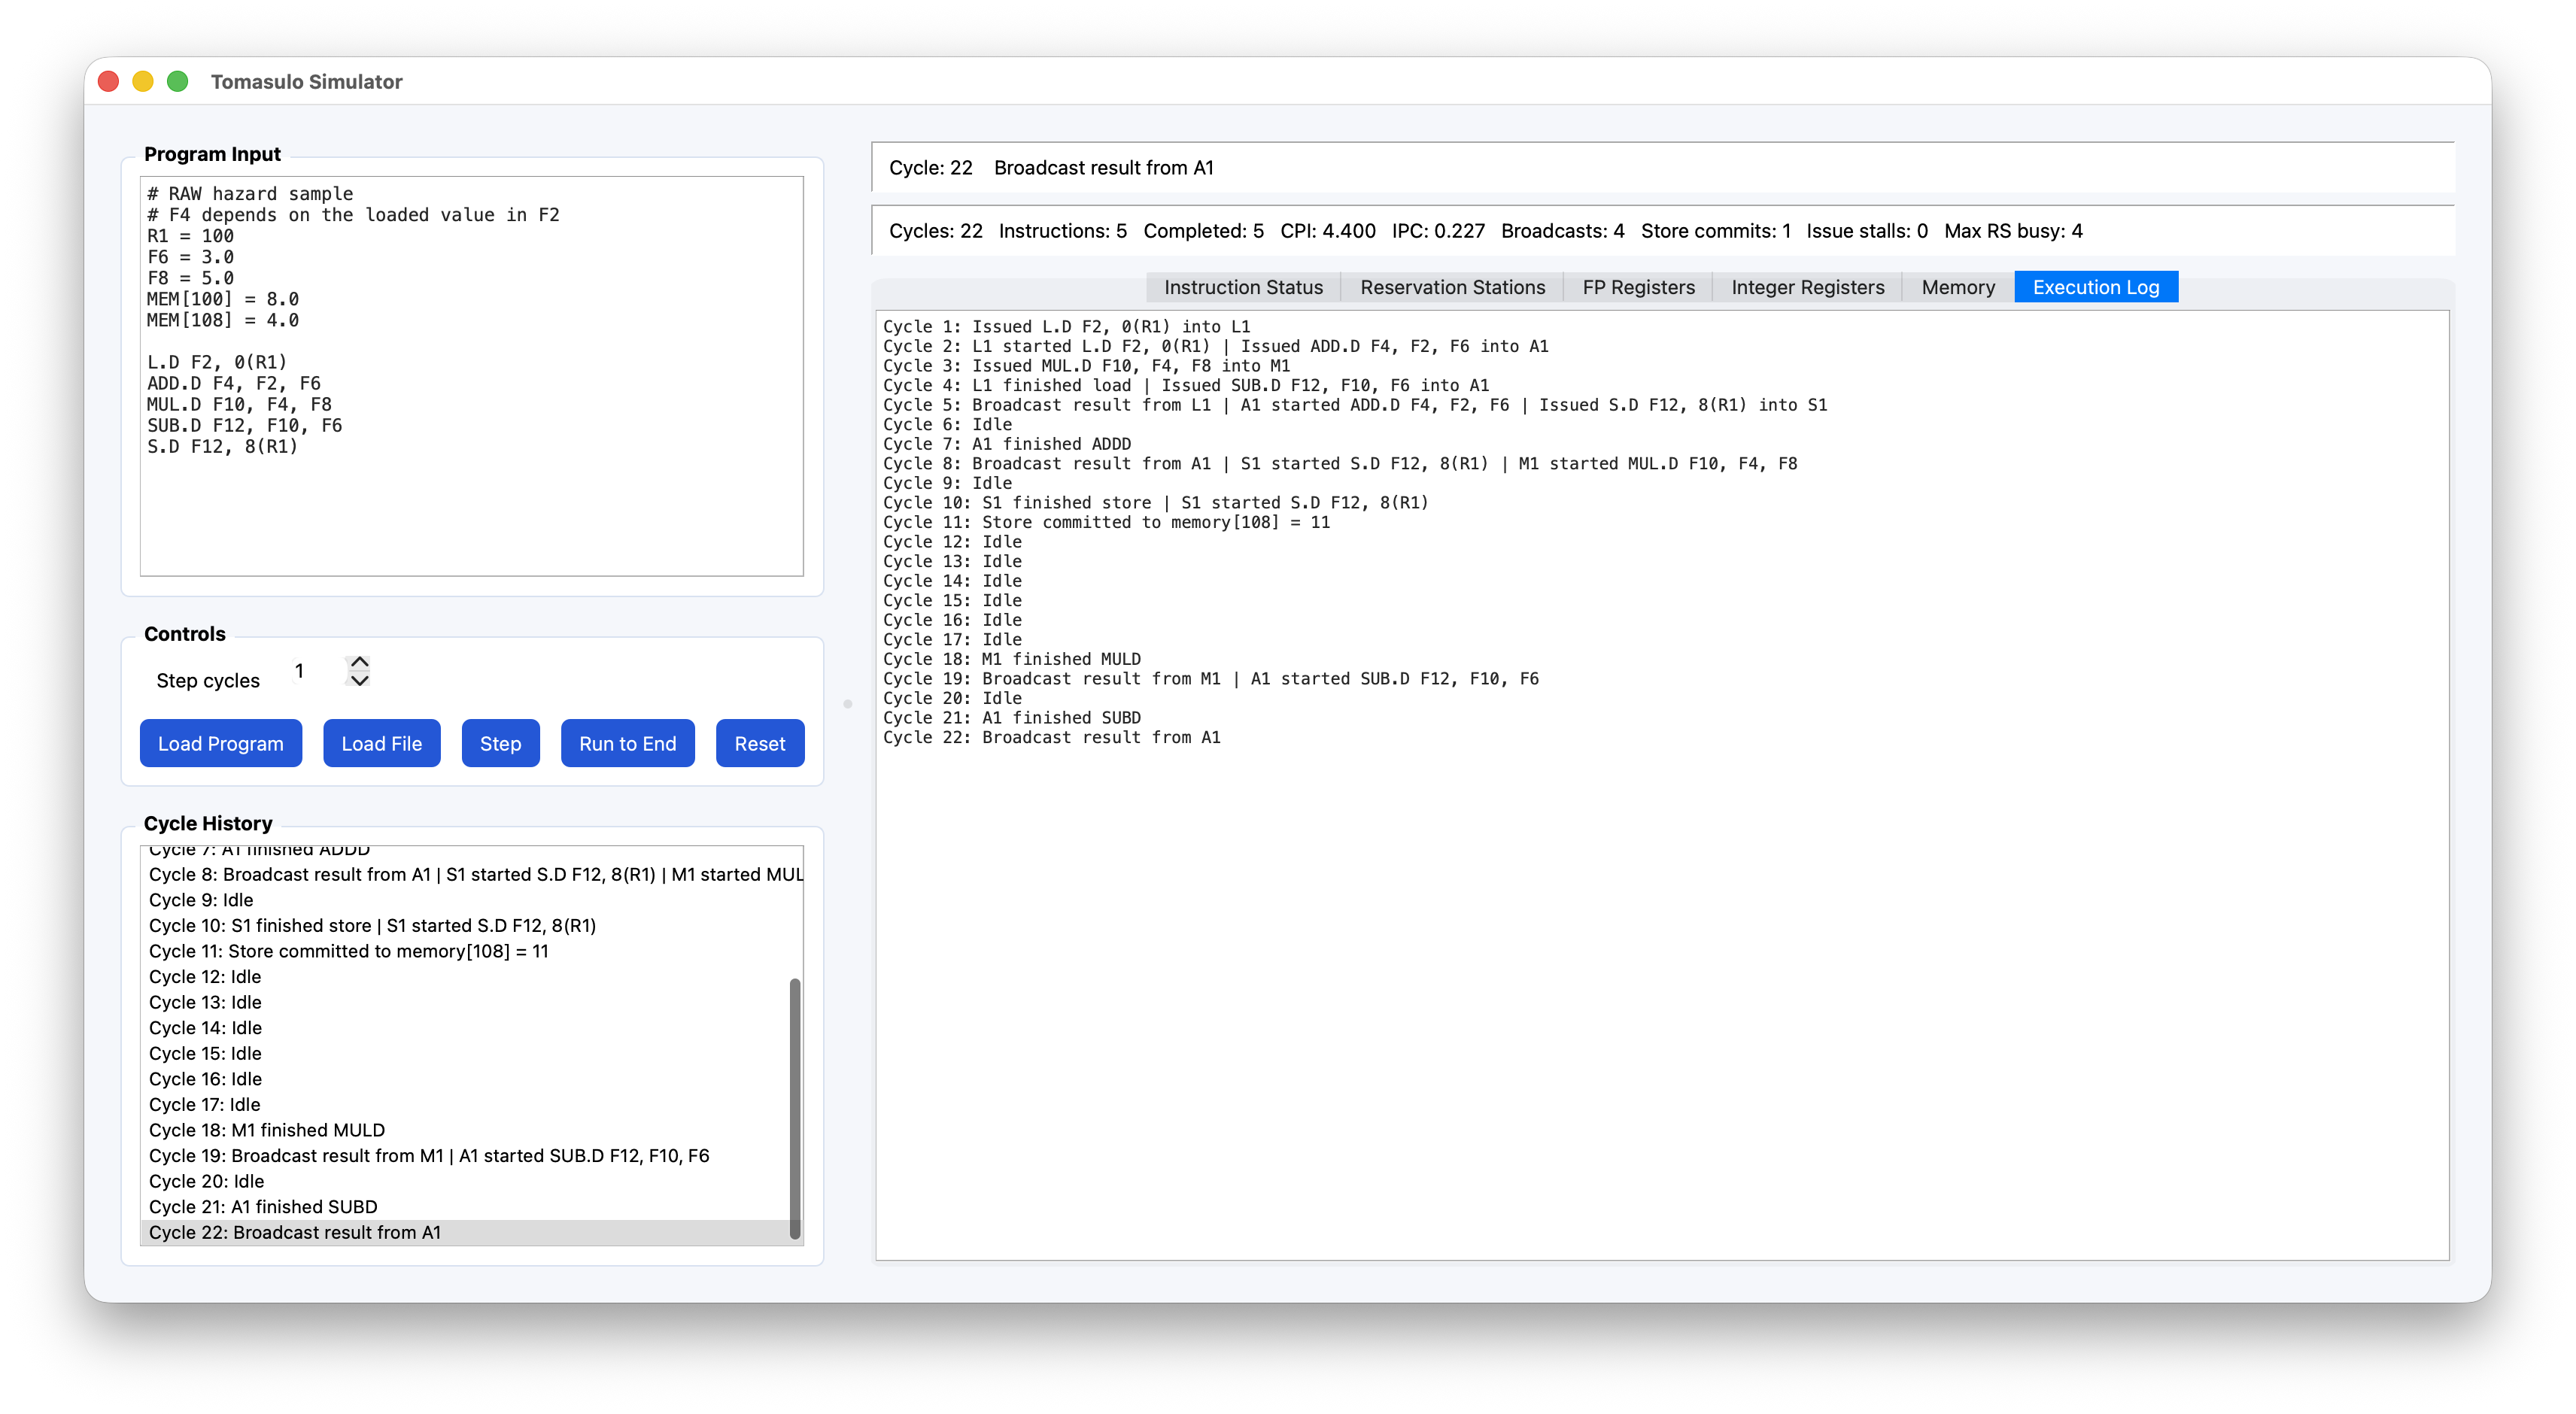
\includegraphics[width=0.8\textwidth]{images/8_raw_hazard_execution.png}
\caption{RAW 示例的执行快照（选取若干周期显示保留站与寄存器变化）}
\end{figure}

\subsection{示例三：写后读（WAR）依赖}
该示例用于演示写后读（Write After Read）依赖：早期指令读取了某寄存器，而后续指令写该寄存器，Tomasulo 通过重命名与保留站解除 WAR 的假依赖。示例代码如下：
\begin{lstlisting}
# WAR hazard sample
# ADD.D reads F2 before a later instruction writes F2
R1 = 100
F2 = 2.0
F4 = 4.0
F6 = 6.0
F8 = 8.0
MEM[100] = 1.0
MEM[108] = 2.0

L.D F10, 0(R1)
ADD.D F12, F2, F4
MUL.D F2, F10, F6
DIV.D F14, F2, F8
S.D F14, 8(R1)
\end{lstlisting}

解释：在这个程序中，ADD.D 在 MUL.D 写回之前读取了旧的 F2 值，Tomasulo 的寄存器状态（register renaming via reservation stations）确保 ADD.D 能获得正确的操作数拷贝，而后续对 F2 的写入不会破坏早先读取的值。对应执行的 GUI 快照示例如下：
\begin{figure}[H]
\centering
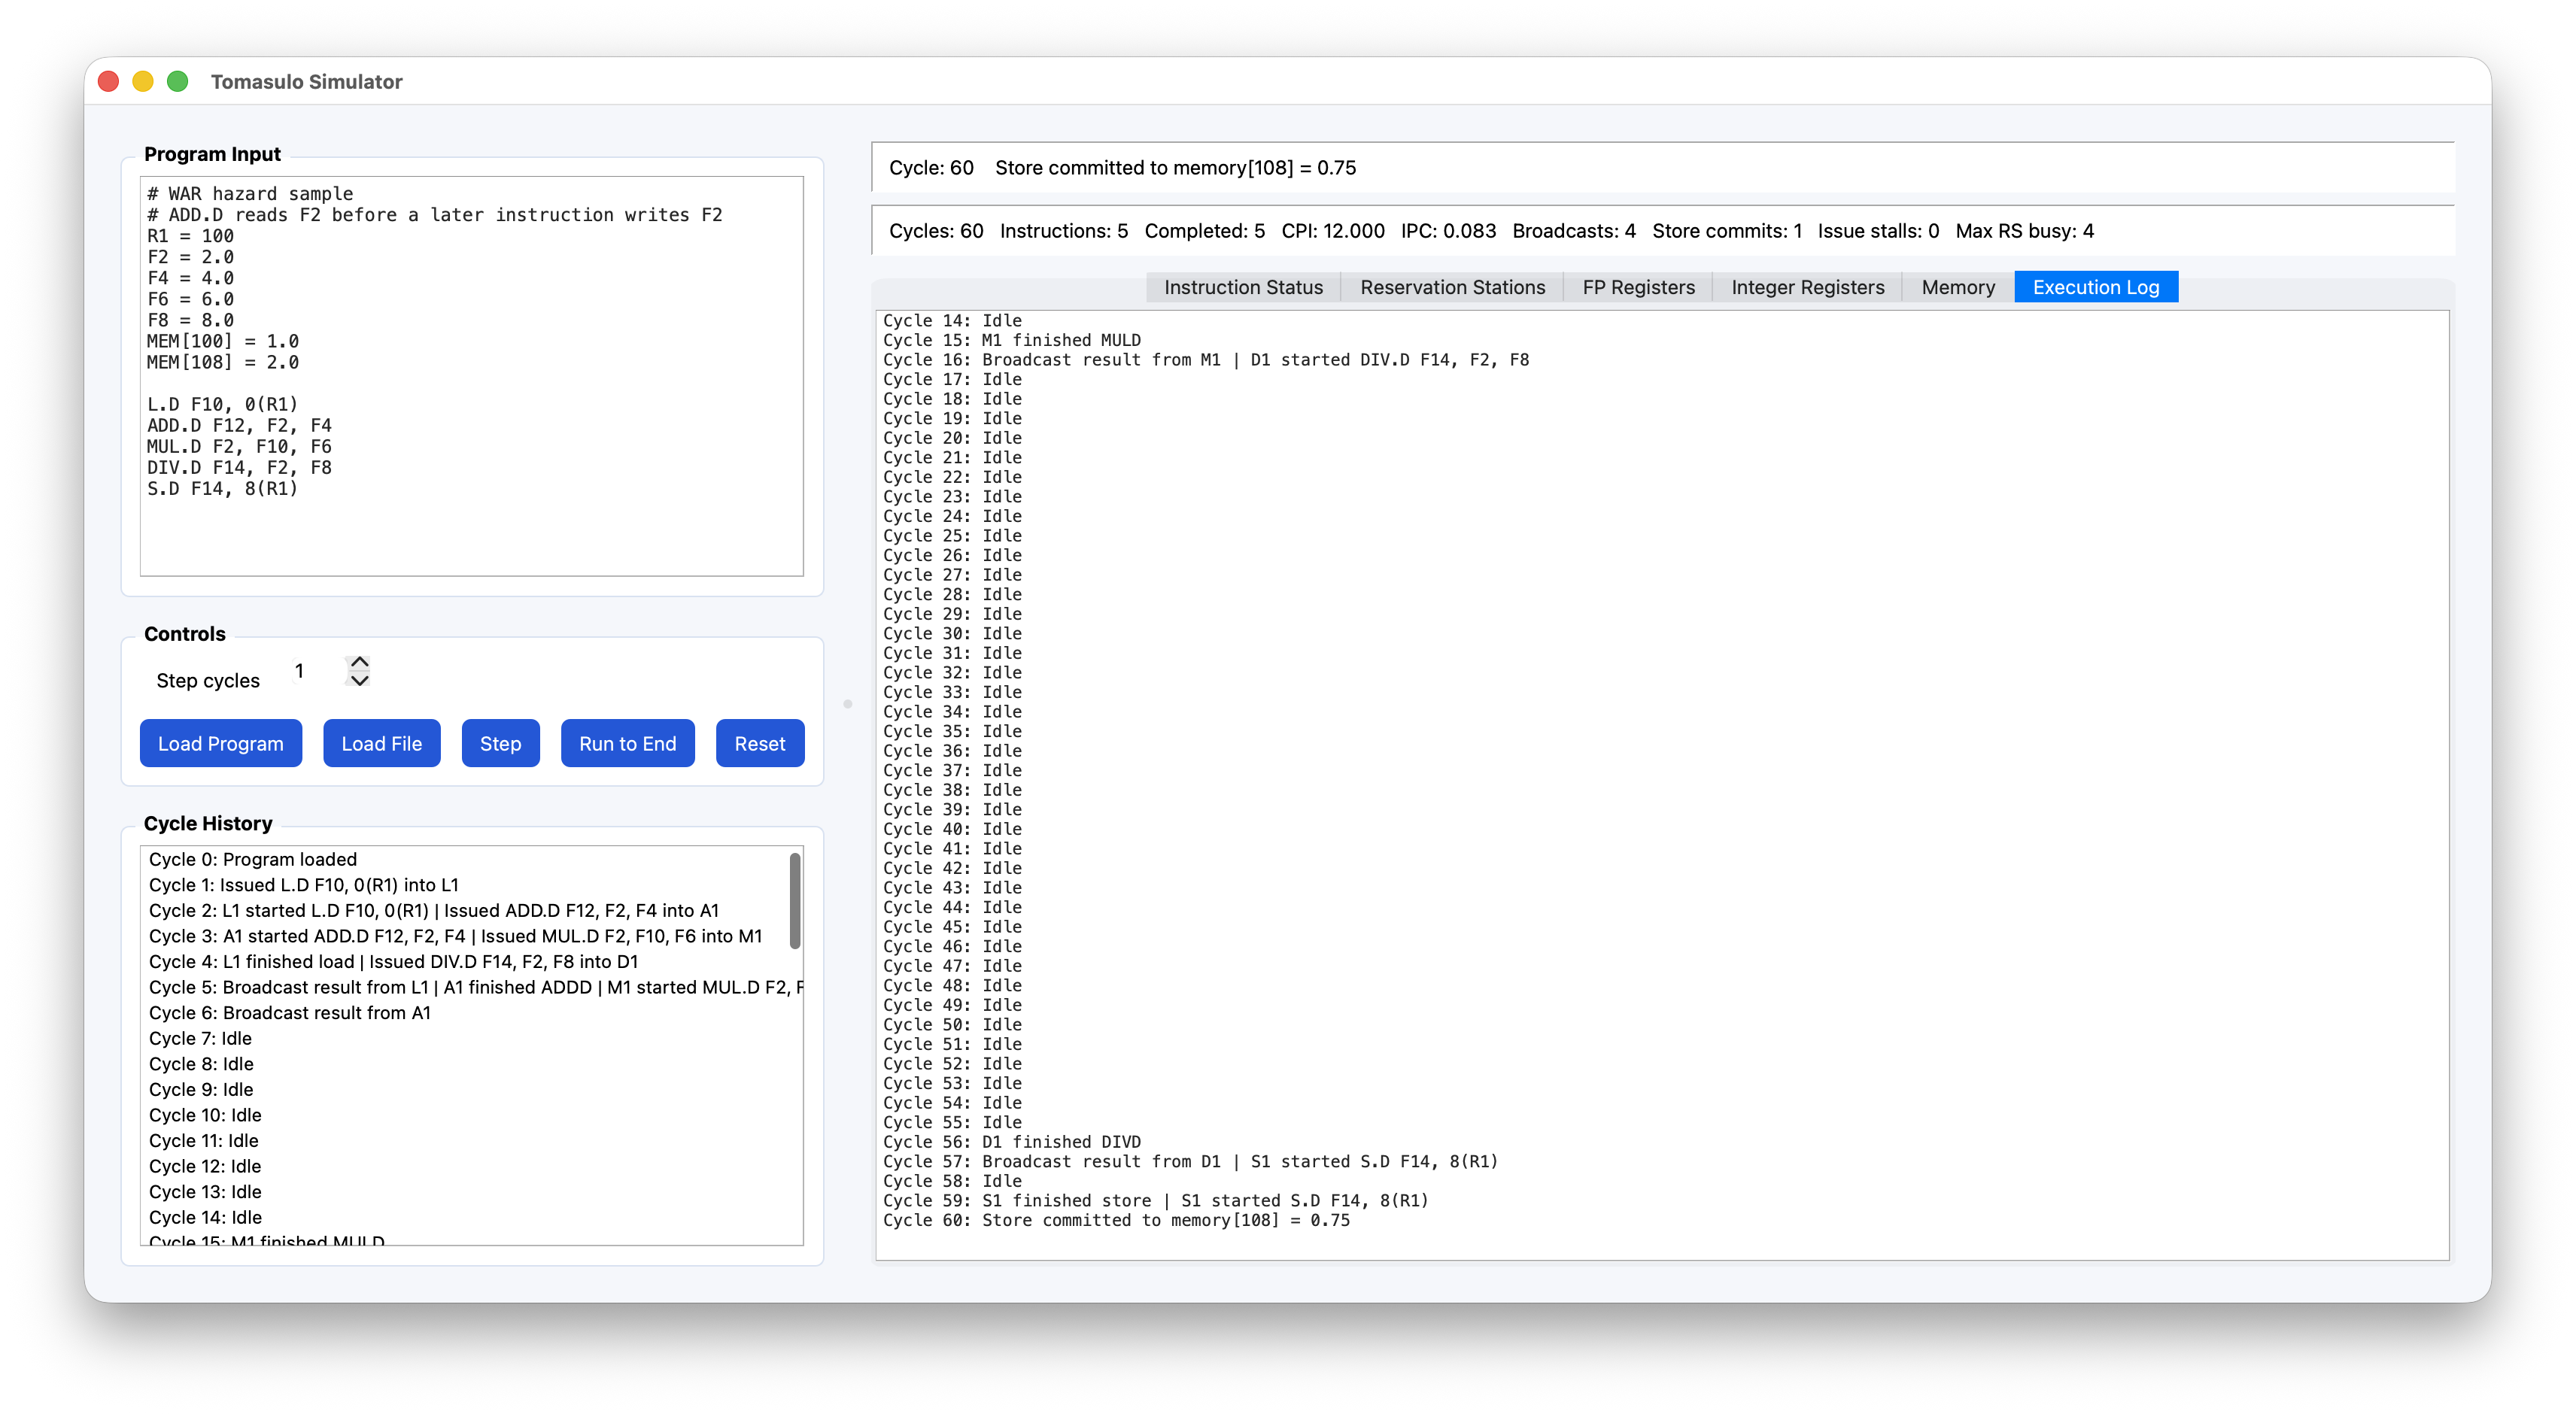
\includegraphics[width=0.8\textwidth]{images/9_war_hazard_execution.png}
\caption{WAR 示例的执行快照（展示读写顺序与保留站状态）}
\end{figure}

\section{实验结果}
针对上述三个示例，我们在仿真器中观察到如下共同特征与统计量：
\begin{itemize}
  \item 在无冲突场景中，多个保留站可以同时占用并并行执行，使 IPC 提高；
  \item 当存在 RAW 依赖时，后续指令将由于等待广播而延迟开始执行或写结果；
  \item Tomasulo 通过对待写寄存器使用保留站标记，以及待广播结果的广播机制来实现分数化重命名，减少 WAR/WAW 的影响；
  \item 仿真器在每周期记录快照，能够回放保留站、指令状态表、寄存器与内存的演化，便于教学与分析。
\end{itemize}

\section{总结}
本实验实现了一个可交互的 Tomasulo 算法仿真器，功能包括：
\begin{itemize}
  \item 支持 MIPS 风格的浮点指令（L.D, S.D, ADD.D, SUB.D, MUL.D, DIV.D）和初始化语句；
  \item 支持单步/多步执行、运行到结束以及历史快照回放；
  \item 可视化保留站、指令状态表、浮点寄存器、整数寄存器与内存；
  \item 提供示例程序演示无冲突、RAW 与 WAR 三类经典场景，并记录统计信息（CPI, IPC, Broadcasts 等）。
\end{itemize}

\section*{附录：实验源代码}
\subsection*{A.1 主要源码：tomasulo_simulator.py}
\begin{lstlisting}
from __future__ import annotations

import argparse
import math
import re
import sys
from dataclasses import dataclass
from pathlib import Path
from typing import Dict, List, Optional, Sequence, Tuple

from PyQt5.QtCore import Qt
from PyQt5.QtGui import QFont, QTextOption
from PyQt5.QtWidgets import (
    QApplication,
    QFileDialog,
    QAbstractItemView,
    QFormLayout,
    QFrame,
    QGroupBox,
    QHBoxLayout,
    QHeaderView,
    QLabel,
    QListWidget,
    QListWidgetItem,
    QMainWindow,
    QMessageBox,
    QPushButton,
    QPlainTextEdit,
    QSpinBox,
    QSplitter,
    QTabWidget,
    QTableWidget,
    QTableWidgetItem,
    QVBoxLayout,
    QWidget,
)

LATENCIES = {
    "LD": 2,
    "SD": 2,
    "ADDD": 2,
    "SUBD": 2,
    "MULD": 10,
    "DIVD": 40,
}

RESERVATION_STATIONS = {
    "LD": ["L1", "L2", "L3"],
    "SD": ["S1", "S2", "S3"],
    "ADDD": ["A1", "A2", "A3"],
    "SUBD": ["A1", "A2", "A3"],
    "MULD": ["M1", "M2"],
    "DIVD": ["D1"],
}


@dataclass
class Instruction:
    index: int
    raw_text: str
    op: str
    dst: Optional[str] = None
    src1: Optional[str] = None
    src2: Optional[str] = None
    base: Optional[str] = None
    offset: int = 0


@dataclass
class InstructionStatus:
    issue: Optional[int] = None
    start_execute: Optional[int] = None
    end_execute: Optional[int] = None
    write_result: Optional[int] = None


@dataclass
class ReservationStation:
    name: str
    kind: str
    busy: bool = False
    op: str = ""
    instruction_index: Optional[int] = None
    instruction_text: str = ""
    remaining: int = 0
    executing: bool = False
    result_ready: bool = False
    result_value: Optional[float] = None
    address: Optional[int] = None
    dest: Optional[str] = None
    Vj: Optional[float] = None
    Vk: Optional[float] = None
    Qj: Optional[str] = None
    Qk: Optional[str] = None
    A: Optional[int] = None

    def reset(self) -> None:
        self.busy = False
        self.op = ""
        self.instruction_index = None
        self.instruction_text = ""
        self.remaining = 0
        self.executing = False
        self.result_ready = False
        self.result_value = None
        self.address = None
        self.dest = None
        self.Vj = None
        self.Vk = None
        self.Qj = None
        self.Qk = None
        self.A = None


@dataclass
class CycleSnapshot:
    cycle: int
    event: str
    instruction_rows: List[Dict[str, str]]
    rs_rows: List[Dict[str, str]]
    fp_register_rows: List[Dict[str, str]]
    int_register_rows: List[Dict[str, str]]
    memory_rows: List[Dict[str, str]]
    stats: Dict[str, str]


def normalize_op(op: str) -> str:
    return re.sub(r"[^A-Z0-9]", "", op.upper())


def normalize_register(token: str) -> str:
    cleaned = token.strip().replace("$", "").upper()
    if cleaned.startswith("F") and cleaned[1:].isdigit():
        return f"F{int(cleaned[1:])}"
    if cleaned.startswith("R") and cleaned[1:].isdigit():
        return f"R{int(cleaned[1:])}"
    raise ValueError(f"Unsupported register: {token}")


def parse_number(text: str) -> float:
    lowered = text.strip().lower()
    if lowered.startswith("0x") or lowered.startswith("-0x"):
        return float(int(lowered, 16))
    if lowered.startswith("0b") or lowered.startswith("-0b"):
        return float(int(lowered, 2))
    return float(text)


def parse_memory_operand(token: str) -> Tuple[int, str]:
    match = re.match(
        r"^([+-]?(?:0x[0-9a-fA-F]+|0b[01]+|\d+(?:\.\d+)?))\(([^)]+)\)$", token.strip()
    )
    if not match:
        raise ValueError(f"Invalid memory operand: {token}")
    offset = int(parse_number(match.group(1)))
    base = normalize_register(match.group(2))
    if not base.startswith("R"):
        raise ValueError(f"Base register must be an integer register: {token}")
    return offset, base


def split_operands(text: str) -> List[str]:
    return [part.strip() for part in text.split(",") if part.strip()]


def format_number(value: Optional[float]) -> str:
    if value is None:
        return ""
    if float(value).is_integer():
        return str(int(value))
    return f"{float(value):.6g}"


class TomasuloSimulator:
    def __init__(self) -> None:
        self.program: List[Instruction] = []
        self.instruction_status: List[InstructionStatus] = []
        self.reservation_stations: List[ReservationStation] = [
            ReservationStation(name=name, kind=kind)
            for kind, names in RESERVATION_STATIONS.items()
            for name in names
        ]
        self.fp_registers: Dict[str, float] = {f"F{i}": 0.0 for i in range(32)}
        self.int_registers: Dict[str, int] = {f"R{i}": 0 for i in range(32)}
        self.register_status: Dict[str, Optional[str]] = {
            f"F{i}": None for i in range(32)
        }
        self.memory: Dict[int, float] = {}
        self.pc = 0
        self.cycle = 0
        self.pending_writes: List[ReservationStation] = []
        self.pending_store_commits: List[ReservationStation] = []
        self.history: List[CycleSnapshot] = []
        self.events: List[str] = []
        self.total_broadcasts = 0
        self.total_store_commits = 0
        self.issue_stalls = 0
        self.max_rs_occupancy = 0

    def reset(self) -> None:
        self.program = []
        self.instruction_status = []
        for station in self.reservation_stations:
            station.reset()
        self.fp_registers = {f"F{i}": 0.0 for i in range(32)}
        self.int_registers = {f"R{i}": 0 for i in range(32)}
        self.register_status = {f"F{i}": None for i in range(32)}
        self.memory = {}
        self.pc = 0
        self.cycle = 0
        self.pending_writes = []
        self.pending_store_commits = []
        self.history = []
        self.events = []
        self.total_broadcasts = 0
        self.total_store_commits = 0
        self.issue_stalls = 0
        self.max_rs_occupancy = 0

    def load_program(self, text: str) -> None:
        self.reset()
        self.program, self.memory, self.int_registers, self.fp_registers = (
            self._parse_source(text)
        )
        self.instruction_status = [InstructionStatus() for _ in self.program]
        self._record_snapshot("Program loaded")

    def _parse_source(
        self, text: str
    ) -> Tuple[List[Instruction], Dict[int, float], Dict[str, int], Dict[str, float]]:
        program: List[Instruction] = []
        memory: Dict[int, float] = {}
        int_registers = {f"R{i}": 0 for i in range(32)}
        fp_registers = {f"F{i}": 0.0 for i in range(32)}

        for line_no, raw_line in enumerate(text.splitlines(), start=1):
            line = re.split(r"(?:#|//|;)", raw_line, maxsplit=1)[0].strip()
            if not line:
                continue
            if ":" in line:
                prefix, remainder = line.split(":", 1)
                if prefix.strip():
                    line = remainder.strip()
                    if not line:
                        continue
            if self._try_parse_initializer(line, memory, int_registers, fp_registers):
                continue
            program.append(self._parse_instruction(line, line_no, len(program)))
        return program, memory, int_registers, fp_registers

    def _try_parse_initializer(
        self,
        line: str,
        memory: Dict[int, float],
        int_registers: Dict[str, int],
        fp_registers: Dict[str, float],
    ) -> bool:
        match = re.match(r"^(MEM|M)\[(.+)\]\s*=\s*(.+)$", line, re.IGNORECASE)
        if match:
            memory[int(parse_number(match.group(2)))] = parse_number(match.group(3))
            return True
        match = re.match(r"^([FR]\d+)\s*=\s*(.+)$", line, re.IGNORECASE)
        if match:
            register = normalize_register(match.group(1))
            value = parse_number(match.group(2))
            if register.startswith("R"):
                int_registers[register] = int(value)
            else:
                fp_registers[register] = float(value)
            return True
        return False

    def _parse_instruction(self, line: str, line_no: int, index: int) -> Instruction:
        match = re.match(r"^([A-Za-z.][A-Za-z0-9.]*)\s*(.*)$", line)
        if not match:
            raise ValueError(f"Cannot parse instruction on line {line_no}: {line}")
        op = normalize_op(match.group(1))
        operands = split_operands(match.group(2).strip())

        if op in {"LD", "LDD"}:
            if len(operands) != 2:
                raise ValueError(f"Invalid load syntax on line {line_no}: {line}")
            dst = normalize_register(operands[0])
            offset, base = parse_memory_operand(operands[1])
            return Instruction(
                index=index, raw_text=line, op="LD", dst=dst, base=base, offset=offset
            )
        if op in {"SD", "STD"}:
            if len(operands) != 2:
                raise ValueError(f"Invalid store syntax on line {line_no}: {line}")
            src = normalize_register(operands[0])
            offset, base = parse_memory_operand(operands[1])
            return Instruction(
                index=index, raw_text=line, op="SD", src1=src, base=base, offset=offset
            )
        if op in {"ADDD", "DADD"}:
            if len(operands) != 3:
                raise ValueError(f"Invalid add.d syntax on line {line_no}: {line}")
            return Instruction(
                index=index,
                raw_text=line,
                op="ADDD",
                dst=normalize_register(operands[0]),
                src1=normalize_register(operands[1]),
                src2=normalize_register(operands[2]),
            )
        if op in {"SUBD", "DSUB"}:
            if len(operands) != 3:
                raise ValueError(f"Invalid sub.d syntax on line {line_no}: {line}")
            return Instruction(
                index=index,
                raw_text=line,
                op="SUBD",
                dst=normalize_register(operands[0]),
                src1=normalize_register(operands[1]),
                src2=normalize_register(operands[2]),
            )
        if op in {"MULD", "MULTD", "DMULT"}:
            if len(operands) != 3:
                raise ValueError(f"Invalid mul.d syntax on line {line_no}: {line}")
            return Instruction(
                index=index,
                raw_text=line,
                op="MULD",
                dst=normalize_register(operands[0]),
                src1=normalize_register(operands[1]),
                src2=normalize_register(operands[2]),
            )
        if op in {"DIVD", "DDIV", "DIV"}:
            if len(operands) != 3:
                raise ValueError(f"Invalid div.d syntax on line {line_no}: {line}")
            return Instruction(
                index=index,
                raw_text=line,
                op="DIVD",
                dst=normalize_register(operands[0]),
                src1=normalize_register(operands[1]),
                src2=normalize_register(operands[2]),
            )
        raise ValueError(f"Unsupported operation on line {line_no}: {line}")

    def has_finished(self) -> bool:
        return (
            self.pc >= len(self.program)
            and not self.pending_writes
            and not self.pending_store_commits
            and all(not station.busy for station in self.reservation_stations)
        )

    def step(self, cycles: int = 1) -> List[str]:
        messages: List[str] = []
        for _ in range(max(1, cycles)):
            if self.has_finished() and self.cycle > 0:
                break
            self.cycle += 1
            cycle_events: List[str] = []
            cycle_events.extend(self._commit_one_store())
            cycle_events.extend(self._broadcast_one())
            cycle_events.extend(self._advance_execution())
            cycle_events.extend(self._start_ready_execution())
            cycle_events.extend(self._issue_one_instruction())
            self.max_rs_occupancy = max(
                self.max_rs_occupancy,
                sum(1 for station in self.reservation_stations if station.busy),
            )
            event_text = " | ".join(cycle_events) if cycle_events else "Idle"
            self.events.append(f"Cycle {self.cycle}: {event_text}")
            self._record_snapshot(event_text)
            messages.append(event_text)
            if self.has_finished():
                break
        return messages

    def run_to_completion(self, max_cycles: int = 10000) -> List[str]:
        messages: List[str] = []
        while not self.has_finished() and self.cycle < max_cycles:
            messages.extend(self.step(1))
        return messages

    def _available_station(self, op: str) -> Optional[ReservationStation]:
        for station in self.reservation_stations:
            if station.kind == op and not station.busy:
                return station
        return None

    def _older_store_blocks_load(self, instruction_index: int, address: int) -> bool:
        for station in self.reservation_stations:
            if (
                station.kind != "SD"
                or not station.busy
                or station.instruction_index is None
                or station.instruction_index >= instruction_index
            ):
                continue
            if station.address is None or station.address == address:
                return True
        return False

    def _older_store_pending(self, instruction_index: int) -> bool:
        for station in self.reservation_stations:
            if (
                station.kind == "SD"
                and station.busy
                and station.instruction_index is not None
                and station.instruction_index < instruction_index
            ):
                return True
        for station in self.pending_store_commits:
            if (
                station.instruction_index is not None
                and station.instruction_index < instruction_index
            ):
                return True
        return False

    def _issue_one_instruction(self) -> List[str]:
        if self.pc >= len(self.program):
            return []
        instruction = self.program[self.pc]
        station = self._available_station(instruction.op)
        if station is None:
            self.issue_stalls += 1
            return [f"Issue stalled for {instruction.raw_text}"]

        if instruction.op == "LD":
            address = self.int_registers[instruction.base] + instruction.offset
            if self._older_store_blocks_load(instruction.index, address):
                self.issue_stalls += 1
                return [f"Issue stalled for {instruction.raw_text}"]

        station.busy = True
        station.op = instruction.op
        station.instruction_index = instruction.index
        station.instruction_text = instruction.raw_text
        station.remaining = LATENCIES[instruction.op]
        station.dest = instruction.dst
        station.A = instruction.offset

        if instruction.op == "LD":
            station.Vj = float(self.int_registers[instruction.base])
            station.address = self.int_registers[instruction.base] + instruction.offset
            if instruction.dst:
                self.register_status[instruction.dst] = station.name
        elif instruction.op == "SD":
            station.Vj = float(self.int_registers[instruction.base])
            station.address = self.int_registers[instruction.base] + instruction.offset
            source_tag = self.register_status[instruction.src1]
            if source_tag is None:
                station.Vk = self.fp_registers[instruction.src1]
            else:
                station.Qk = source_tag
        else:
            source1_tag = self.register_status[instruction.src1]
            source2_tag = self.register_status[instruction.src2]
            if source1_tag is None:
                station.Vj = self.fp_registers[instruction.src1]
            else:
                station.Qj = source1_tag
            if source2_tag is None:
                station.Vk = self.fp_registers[instruction.src2]
            else:
                station.Qk = source2_tag
            if instruction.dst:
                self.register_status[instruction.dst] = station.name

        self.instruction_status[instruction.index].issue = self.cycle
        self.pc += 1
        return [f"Issued {instruction.raw_text} into {station.name}"]

    def _start_ready_execution(self) -> List[str]:
        messages: List[str] = []
        for station in self.reservation_stations:
            if (
                not station.busy
                or station.executing
                or station.result_ready
                or station.instruction_index is None
            ):
                continue
            if station.kind == "LD" and station.Qj is None:
                station.executing = True
            elif (
                station.kind == "SD"
                and station.Qk is None
                and not self._older_store_pending(station.instruction_index)
            ):
                station.executing = True
            elif (
                station.kind in {"ADDD", "SUBD", "MULD", "DIVD"}
                and station.Qj is None
                and station.Qk is None
            ):
                station.executing = True
            else:
                continue

            self.instruction_status[station.instruction_index].start_execute = (
                self.cycle
            )
            messages.append(f"{station.name} started {station.instruction_text}")
        return messages

    def _advance_execution(self) -> List[str]:
        messages: List[str] = []
        for station in self.reservation_stations:
            if not station.busy or not station.executing:
                continue
            station.remaining -= 1
            if station.remaining > 0:
                continue
            station.executing = False
            self.instruction_status[station.instruction_index].end_execute = self.cycle
            if station.kind == "LD":
                station.result_value = self.memory.get(int(station.address or 0), 0.0)
                station.result_ready = True
                self.pending_writes.append(station)
                messages.append(f"{station.name} finished load")
            elif station.kind == "SD":
                self.pending_store_commits.append(station)
                messages.append(f"{station.name} finished store")
            else:
                left = float(station.Vj or 0.0)
                right = float(station.Vk or 0.0)
                if station.op == "ADDD":
                    station.result_value = left + right
                elif station.op == "SUBD":
                    station.result_value = left - right
                elif station.op == "MULD":
                    station.result_value = left * right
                elif station.op == "DIVD":
                    station.result_value = left / right if right != 0 else float("inf")
                station.result_ready = True
                self.pending_writes.append(station)
                messages.append(f"{station.name} finished {station.op}")
        return messages

    def _broadcast_one(self) -> List[str]:
        if not self.pending_writes:
            return []
        station = self.pending_writes.pop(0)
        if not station.busy or not station.result_ready:
            return []
        if station.dest and self.register_status.get(station.dest) == station.name:
            self.fp_registers[station.dest] = float(station.result_value or 0.0)
            self.register_status[station.dest] = None
        for waiting_station in self.reservation_stations:
            if waiting_station.Qj == station.name:
                waiting_station.Qj = None
                waiting_station.Vj = float(station.result_value or 0.0)
            if waiting_station.Qk == station.name:
                waiting_station.Qk = None
                waiting_station.Vk = float(station.result_value or 0.0)
        self.instruction_status[station.instruction_index].write_result = self.cycle
        self.total_broadcasts += 1
        station.reset()
        return [f"Broadcast result from {station.name}"]

    def _commit_one_store(self) -> List[str]:
        if not self.pending_store_commits:
            return []
        self.pending_store_commits.sort(
            key=lambda item: (
                item.instruction_index if item.instruction_index is not None else 10**9
            )
        )
        for position, station in enumerate(self.pending_store_commits):
            if station.instruction_index is None or self._older_store_pending(
                station.instruction_index
            ):
                continue
            address = int(station.address or 0)
            self.memory[address] = float(station.Vk or 0.0)
            self.instruction_status[station.instruction_index].write_result = self.cycle
            self.total_store_commits += 1
            self.pending_store_commits.pop(position)
            station.reset()
            return [
                f"Store committed to memory[{address}] = {format_number(self.memory[address])}"
            ]
        return []

    def _record_snapshot(self, event: str) -> None:
        self.history.append(
            CycleSnapshot(
                cycle=self.cycle,
                event=event,
                instruction_rows=self._build_instruction_rows(),
                rs_rows=self._build_rs_rows(),
                fp_register_rows=self._build_fp_rows(),
                int_register_rows=self._build_int_rows(),
                memory_rows=self._build_memory_rows(),
                stats=self._build_stats(),
            )
        )

    def _build_instruction_rows(self) -> List[Dict[str, str]]:
        rows: List[Dict[str, str]] = []
        for instruction, status in zip(self.program, self.instruction_status):
            rows.append(
                {
                    "Instruction": instruction.raw_text,
                    "Issue": "" if status.issue is None else str(status.issue),
                    "Start": (
                        ""
                        if status.start_execute is None
                        else str(status.start_execute)
                    ),
                    "End": (
                        "" if status.end_execute is None else str(status.end_execute)
                    ),
                    "Write": (
                        "" if status.write_result is None else str(status.write_result)
                    ),
                }
            )
        return rows

    def _build_rs_rows(self) -> List[Dict[str, str]]:
        rows: List[Dict[str, str]] = []
        for station in self.reservation_stations:
            rows.append(
                {
                    "Name": station.name,
                    "Busy": "Yes" if station.busy else "No",
                    "Op": station.op,
                    "Vj": format_number(station.Vj),
                    "Vk": format_number(station.Vk),
                    "Qj": station.Qj or "",
                    "Qk": station.Qk or "",
                    "A": "" if station.A is None else str(station.A),
                    "Dest": station.dest or "",
                    "Rem": "" if not station.busy else str(station.remaining),
                }
            )
        return rows

    def _build_fp_rows(self) -> List[Dict[str, str]]:
        rows: List[Dict[str, str]] = []
        for index in range(32):
            register = f"F{index}"
            rows.append(
                {
                    "Register": register,
                    "Value": format_number(self.fp_registers[register]),
                    "Status": self.register_status[register] or "",
                }
            )
        return rows

    def _build_int_rows(self) -> List[Dict[str, str]]:
        rows: List[Dict[str, str]] = []
        for index in range(32):
            register = f"R{index}"
            rows.append(
                {"Register": register, "Value": str(self.int_registers[register])}
            )
        return rows

    def _build_memory_rows(self) -> List[Dict[str, str]]:
        return [
            {"Address": str(address), "Value": format_number(self.memory[address])}
            for address in sorted(self.memory)
        ]

    def _build_stats(self) -> Dict[str, str]:
        completed = sum(
            1 for status in self.instruction_status if status.write_result is not None
        )
        cpi = self.cycle / completed if completed else 0.0
        ipc = completed / self.cycle if self.cycle else 0.0
        return {
            "Cycles": str(self.cycle),
            "Instructions": str(len(self.program)),
            "Completed": str(completed),
            "CPI": f"{cpi:.3f}" if completed else "0.000",
            "IPC": f"{ipc:.3f}" if self.cycle else "0.000",
            "Broadcasts": str(self.total_broadcasts),
            "Store commits": str(self.total_store_commits),
            "Issue stalls": str(self.issue_stalls),
            "Max RS busy": str(self.max_rs_occupancy),
        }


def populate_table(
    table: QTableWidget, rows: List[Dict[str, str]], headers: Sequence[str]
) -> None:
    table.clear()
    table.setColumnCount(len(headers))
    table.setRowCount(len(rows))
    table.setHorizontalHeaderLabels(list(headers))
    for row_index, row in enumerate(rows):
        for column_index, header in enumerate(headers):
            table.setItem(
                row_index, column_index, QTableWidgetItem(row.get(header, ""))
            )
    table.resizeColumnsToContents()


class TableView(QTableWidget):
    def __init__(self) -> None:
        super().__init__()
        self.setAlternatingRowColors(True)
        self.setEditTriggers(QAbstractItemView.NoEditTriggers)
        self.horizontalHeader().setSectionResizeMode(QHeaderView.ResizeToContents)
        self.horizontalHeader().setStretchLastSection(True)
        self.verticalHeader().setVisible(False)


class TomasuloWindow(QMainWindow):
    def __init__(self) -> None:
        super().__init__()
        self.setWindowTitle("Tomasulo Simulator")
        self.resize(1600, 960)
        self.simulator = TomasuloSimulator()
        self._build_ui()
        self._load_default_example()

    def _build_ui(self) -> None:
        central = QWidget()
        self.setCentralWidget(central)
        main_layout = QHBoxLayout(central)
        splitter = QSplitter(Qt.Horizontal)
        main_layout.addWidget(splitter)

        left_panel = QWidget()
        left_layout = QVBoxLayout(left_panel)

        input_group = QGroupBox("Program Input")
        input_layout = QVBoxLayout(input_group)
        self.program_editor = QPlainTextEdit()
        self.program_editor.setWordWrapMode(QTextOption.NoWrap)
        self.program_editor.setFont(QFont("Menlo", 12))
        input_layout.addWidget(self.program_editor)
        left_layout.addWidget(input_group, stretch=1)

        controls_group = QGroupBox("Controls")
        controls_layout = QFormLayout(controls_group)
        self.step_spin = QSpinBox()
        self.step_spin.setRange(1, 1000)
        self.step_spin.setValue(1)
        controls_layout.addRow("Step cycles", self.step_spin)

        button_row = QWidget()
        button_row_layout = QHBoxLayout(button_row)
        button_row_layout.setContentsMargins(0, 0, 0, 0)
        self.load_button = QPushButton("Load Program")
        self.file_button = QPushButton("Load File")
        self.step_button = QPushButton("Step")
        self.run_button = QPushButton("Run to End")
        self.reset_button = QPushButton("Reset")
        for button in [
            self.load_button,
            self.file_button,
            self.step_button,
            self.run_button,
            self.reset_button,
        ]:
            button_row_layout.addWidget(button)
        controls_layout.addRow(button_row)
        left_layout.addWidget(controls_group)

        history_group = QGroupBox("Cycle History")
        history_layout = QVBoxLayout(history_group)
        self.history_list = QListWidget()
        self.history_list.currentRowChanged.connect(self.on_history_selected)
        history_layout.addWidget(self.history_list)
        left_layout.addWidget(history_group, stretch=1)

        splitter.addWidget(left_panel)

        right_panel = QWidget()
        right_layout = QVBoxLayout(right_panel)
        self.cycle_label = QLabel("Cycle: 0")
        self.cycle_label.setFrameShape(QFrame.Panel)
        self.cycle_label.setFrameShadow(QFrame.Sunken)
        right_layout.addWidget(self.cycle_label)

        self.stats_label = QLabel("")
        self.stats_label.setWordWrap(True)
        self.stats_label.setFrameShape(QFrame.Panel)
        self.stats_label.setFrameShadow(QFrame.Sunken)
        right_layout.addWidget(self.stats_label)

        tabs = QTabWidget()
        self.instruction_table = TableView()
        self.rs_table = TableView()
        self.fp_table = TableView()
        self.int_table = TableView()
        self.memory_table = TableView()
        self.log_view = QPlainTextEdit()
        self.log_view.setReadOnly(True)
        self.log_view.setWordWrapMode(QTextOption.NoWrap)
        self.log_view.setFont(QFont("Menlo", 11))
        tabs.addTab(self.instruction_table, "Instruction Status")
        tabs.addTab(self.rs_table, "Reservation Stations")
        tabs.addTab(self.fp_table, "FP Registers")
        tabs.addTab(self.int_table, "Integer Registers")
        tabs.addTab(self.memory_table, "Memory")
        tabs.addTab(self.log_view, "Execution Log")
        right_layout.addWidget(tabs, stretch=1)

        splitter.addWidget(right_panel)
        splitter.setStretchFactor(0, 1)
        splitter.setStretchFactor(1, 2)

        self.setStyleSheet("""
            QMainWindow { background: #f5f7fb; }
            QGroupBox { font-weight: 600; border: 1px solid #d9e2f1; border-radius: 6px; margin-top: 10px; background: white; }
            QGroupBox::title { subcontrol-origin: margin; left: 10px; padding: 0 4px; }
            QPushButton { padding: 8px 12px; border-radius: 6px; background: #2457d6; color: white; }
            QPushButton:hover { background: #1f49b3; }
            QPushButton:pressed { background: #17398d; }
            QPlainTextEdit, QListWidget, QTableWidget, QLabel { background: white; }
            QLabel { padding: 8px; }
            """)

        self.load_button.clicked.connect(self.load_program_from_editor)
        self.file_button.clicked.connect(self.load_program_from_file)
        self.step_button.clicked.connect(self.step_cycles)
        self.run_button.clicked.connect(self.run_to_end)
        self.reset_button.clicked.connect(self.reset_view)

    def _load_default_example(self) -> None:
        self.program_editor.setPlainText("""# Supported initialization examples
R1 = 100
F0 = 1.0
F2 = 3.0
MEM[100] = 8.0
MEM[108] = 2.0

L.D F6, 0(R1)
ADD.D F8, F6, F2
MUL.D F10, F8, F2
S.D F10, 8(R1)
DIV.D F12, F10, F2
SUB.D F14, F12, F0
""")
        self._load_into_simulator(self.program_editor.toPlainText())

    def _load_into_simulator(self, text: str) -> None:
        try:
            self.simulator.load_program(text)
        except Exception as exc:  # noqa: BLE001
            QMessageBox.critical(self, "Load Error", str(exc))
            return
        self._refresh_all_views()

    def load_program_from_editor(self) -> None:
        self._load_into_simulator(self.program_editor.toPlainText())

    def load_program_from_file(self) -> None:
        path, _ = QFileDialog.getOpenFileName(
            self,
            "Open Program",
            str(Path.home()),
            "Assembly Files (*.asm *.s *.txt);;All Files (*)",
        )
        if not path:
            return
        try:
            text = Path(path).read_text(encoding="utf-8")
        except UnicodeDecodeError:
            text = Path(path).read_text(encoding="utf-8-sig")
        except Exception as exc:  # noqa: BLE001
            QMessageBox.critical(self, "File Error", str(exc))
            return
        self.program_editor.setPlainText(text)
        self._load_into_simulator(text)

    def step_cycles(self) -> None:
        if not self.simulator.program:
            self.load_program_from_editor()
            if not self.simulator.program:
                return
        self.simulator.step(self.step_spin.value())
        self._refresh_all_views()

    def run_to_end(self) -> None:
        if not self.simulator.program:
            self.load_program_from_editor()
            if not self.simulator.program:
                return
        self.simulator.run_to_completion()
        self._refresh_all_views()

    def reset_view(self) -> None:
        self._load_default_example()

    def on_history_selected(self, row: int) -> None:
        if row < 0 or row >= len(self.simulator.history):
            return
        self._render_snapshot(self.simulator.history[row])

    def _refresh_all_views(self) -> None:
        self.history_list.blockSignals(True)
        self.history_list.clear()
        for snapshot in self.simulator.history:
            self.history_list.addItem(
                QListWidgetItem(f"Cycle {snapshot.cycle}: {snapshot.event}")
            )
        self.history_list.blockSignals(False)
        if self.simulator.history:
            self.history_list.setCurrentRow(len(self.simulator.history) - 1)
            self._render_snapshot(self.simulator.history[-1])

    def _render_snapshot(self, snapshot: CycleSnapshot) -> None:
        populate_table(
            self.instruction_table,
            snapshot.instruction_rows,
            ["Instruction", "Issue", "Start", "End", "Write"],
        )
        populate_table(
            self.rs_table,
            snapshot.rs_rows,
            ["Name", "Busy", "Op", "Vj", "Vk", "Qj", "Qk", "A", "Dest", "Rem"],
        )
        populate_table(
            self.fp_table, snapshot.fp_register_rows, ["Register", "Value", "Status"]
        )
        populate_table(
            self.int_table, snapshot.int_register_rows, ["Register", "Value"]
        )
        populate_table(self.memory_table, snapshot.memory_rows, ["Address", "Value"])
        self.cycle_label.setText(f"Cycle: {snapshot.cycle}    {snapshot.event}")
        self.stats_label.setText(
            "   ".join(f"{key}: {value}" for key, value in snapshot.stats.items())
        )
        self.log_view.setPlainText(
            "\n".join(self.simulator.events)
            if self.simulator.events
            else "No activity yet."
        )


def main(argv: Optional[Sequence[str]] = None) -> int:
    parser = argparse.ArgumentParser(description="PyQt5 Tomasulo simulator")
    parser.add_argument("--file", help="Load program file at startup")
    args = parser.parse_args(argv)

    app = QApplication(list(argv) if argv is not None else sys.argv)
    window = TomasuloWindow()
    if args.file:
        path = Path(args.file)
        if path.exists():
            window.program_editor.setPlainText(path.read_text(encoding="utf-8"))
            window.load_program_from_editor()
    window.show()
    return app.exec_()


if __name__ == "__main__":
    raise SystemExit(main())
\end{lstlisting}

\subsection*{A.2 本次实验的示例程序}
\paragraph{示例：no_hazard.asm}
\begin{lstlisting}
# No hazard sample
# Independent operations to demonstrate a clean Tomasulo schedule
R1 = 100
F0 = 1.0
F2 = 2.0
F4 = 3.0
F6 = 4.0
F8 = 5.0
F10 = 6.0
F12 = 7.0
MEM[100] = 11.0
MEM[108] = 22.0
MEM[116] = 33.0

L.D F14, 0(R1)
L.D F16, 8(R1)
ADD.D F18, F2, F4
SUB.D F20, F6, F0
MUL.D F22, F8, F10
DIV.D F24, F12, F2
S.D F14, 16(R1)
\end{lstlisting}

\paragraph{示例：raw_hazard.asm}
\begin{lstlisting}
# RAW hazard sample
# F4 depends on the loaded value in F2
R1 = 100
F6 = 3.0
F8 = 5.0
MEM[100] = 8.0
MEM[108] = 4.0

L.D F2, 0(R1)
ADD.D F4, F2, F6
MUL.D F10, F4, F8
SUB.D F12, F10, F6
S.D F12, 8(R1)
\end{lstlisting}

\paragraph{示例：war_hazard.asm}
\begin{lstlisting}
# WAR hazard sample
# ADD.D reads F2 before a later instruction writes F2
R1 = 100
F2 = 2.0
F4 = 4.0
F6 = 6.0
F8 = 8.0
MEM[100] = 1.0
MEM[108] = 2.0

L.D F10, 0(R1)
ADD.D F12, F2, F4
MUL.D F2, F10, F6
DIV.D F14, F2, F8
S.D F14, 8(R1)
\end{lstlisting}

\subsection*{A.3 运行说明}
在包含依赖的 Python 环境中，运行如下命令启动 GUI：
\begin{verbatim}
# 安装依赖（示例）
pip install -r requirements.txt

# 启动仿真器
python tomasulo_simulator.py

# 或者直接指定程序文件启动
python tomasulo_simulator.py --file examples/no_hazard.asm
\end{verbatim}

\end{document}
